\section{Combination of \acs*{SEM}-\acs*{BSE} + \acs*{EDX} + \acs*{LAICPMS} }
\label{sec:corr_laicpms}

%TODO: Why are trace elements interesting for clinker:
% \cite{miliszkiewicz.2015} Current approaches to calibration of LA-ICP-MS analysis

\textit{The results of this section are published in \cite{kleiner.2022b}. However, another area of the specimen was chosen to discuss the results.}

The production of cement clinker has a high carbon footprint.
To reduce this footprint, alternative fuels and raw materials, which are often industrial waste products, are used to reduce the primary energy usage and preserve natural resources \cite{schneider.2015}.
This practice inherently causes the entry of minor (<\,\qtyrange{1.0}{2.0}{\wtpercent}) and trace elements (<\,\qty{0.1}{\wtpercent}) into the kiln system and ultimately into the final clinker product \cite{stephan.1999,barros.2004,thiery.2025}.
Determining the exact spatial distribution and phase-specific incorporation of these trace elements is of great scientific and practical interest.
Depending on their specific ionic radius and charge, trace elements are preferentially incorporated into certain clinker phases.
There, they can substitute host ions, distort the crystal lattice, stabilise specific high-temperature polymorphs, and alter the viscosity of the clinker melt.
This, in turn, can significantly affect the hydraulic reactivity and the strength development of the resulting cement \cite{stephan.1999, barros.2004, stephan.2006, ludwig.2015}.
Furthermore, understanding the exact phase association of potentially hazardous heavy metals is crucial for evaluating their immobilisation and long-term leaching behaviour in the hardened concrete \cite{achternbosch.2003, kolovos.2002}.

The experiments were carried out on an embedded and polished clinker grain (composition, see \zcref{tab:phase-composition-clinker}).
The measurement areas are visible as dark spots (\zcref{fig:LAICPMS-specimen}), already indicating a damage induced by the laser ablation.
In total, there were three mapping areas and one spot analysis area, which was fully evaluated in \cite{kleiner.2022b}.

The evaluation is described using one mapping position as an example.
\zcref{fig:LAICPMS-position2} shows the area of the \ac{EDX} mapping and the subsequent \ac{LAICPMS} area on top of a \ac{BSE} image.

\begin{figure}[htb!]
  \centering

  \begin{subfigure}[t]{0.49\textwidth}
      \ifdefined\PRINTABLE
        \includegraphics[width=\linewidth]{la-icp-ms/position2.pdf}
      \else
        \animategraphics[loop,autoplay,width=\linewidth]{.5}{figures/la-icp-ms/position2-anim/Animation}{0}{4}
      \fi
    \caption{Data positioning}
    \label{fig:LAICPMS-positions}
  \end{subfigure}
  \hfill
  \begin{subfigure}[t]{0.49\textwidth}
    \includegraphics[width=\textwidth]{la-icp-ms/LA-BSE.pdf}
    \caption{\ac{BSE} image of the \ac{LAICPMS}-induced damage.}
    \label{fig:LAICPMS-site-damage}
  \end{subfigure}

  \caption{
    Position of the \ce{Si}-\ac{EDX}- ({\color{red}red}) and \ce{Ba}-\ac{LAICPMS}-mapping ({\color{orange}yellow}). \cite{kleiner.2021d, kleiner.2022b}
  }
  \label{fig:LAICPMS-position2}
\end{figure}

The areas measured contain all relevant phases, such as \ac{C3S}, \ac{C2S}, \ac{C3A}, \ac{C4AF}, \ce{MgO}, \ce{CaO}, and alkali sulphates.
\ac{C3S} and \ac{C2S} are easily identifiable in the \ac{BSE} image (\ac{C2S} appears a little darker than \ac{C3S}), but also in the \ac{EDX} mappings.
Selected \ac{EDX} element distribution maps are presented in \zcref{fig:LAICPMS-EDX}.

\begin{figure}[htb]
  \centering

  \begin{subfigure}[t]{0.32\textwidth}
    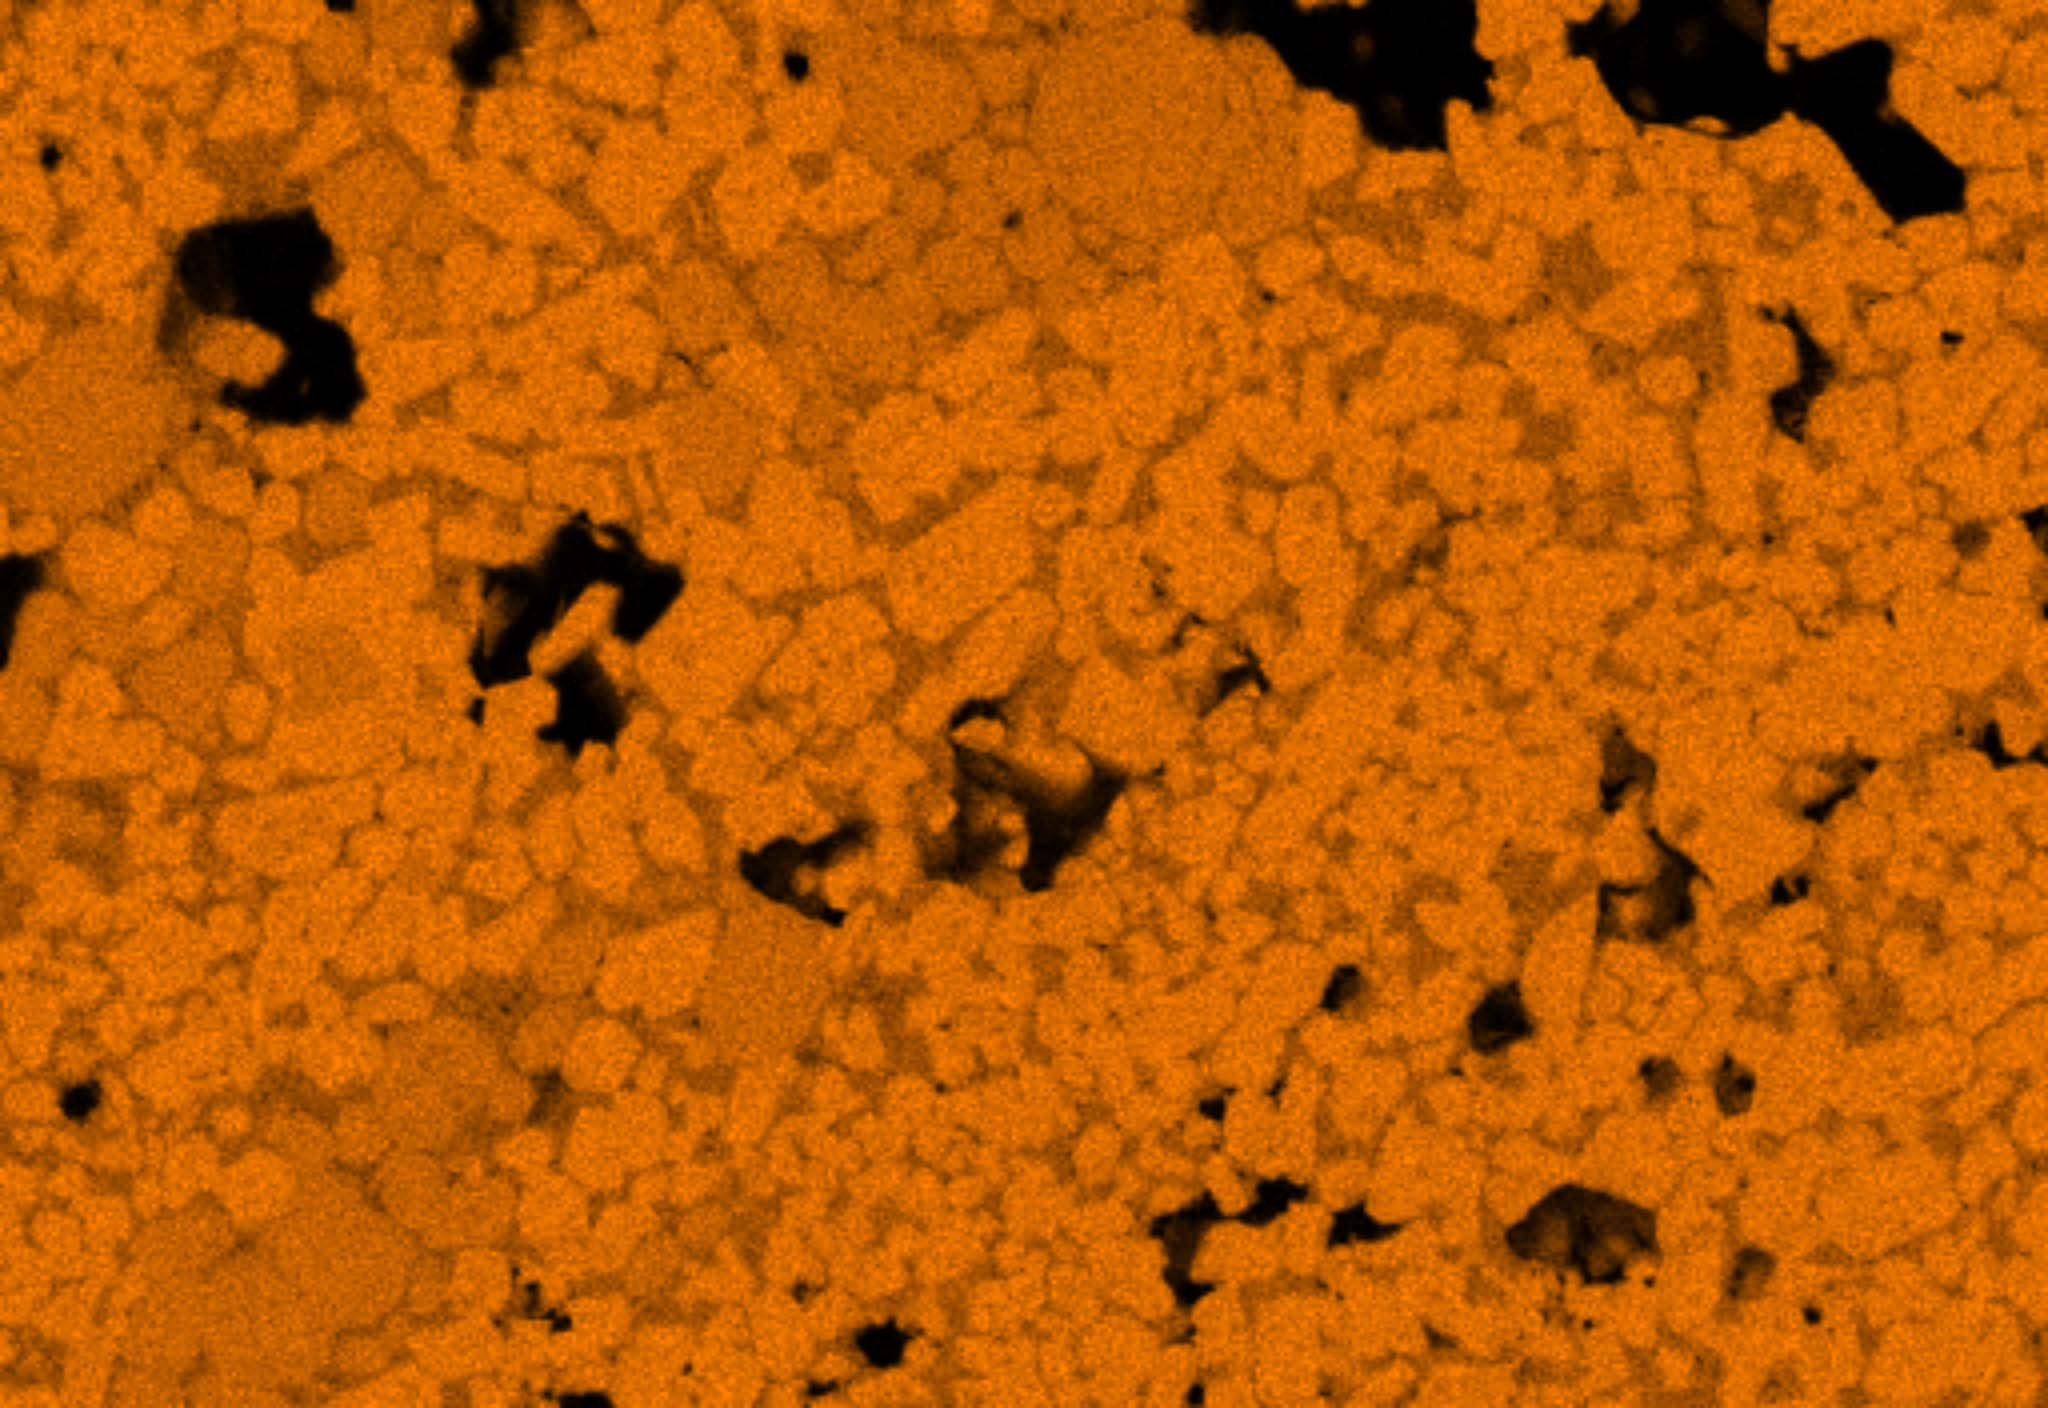
\includegraphics[width=\textwidth]{figures/la-icp-ms/edx/Ca.jpg}
    \caption{Ca mapping}
    \label{fig:LAICPMS-EDX-Ca}
  \end{subfigure}
  \hfill
  \begin{subfigure}[t]{0.32\textwidth}
    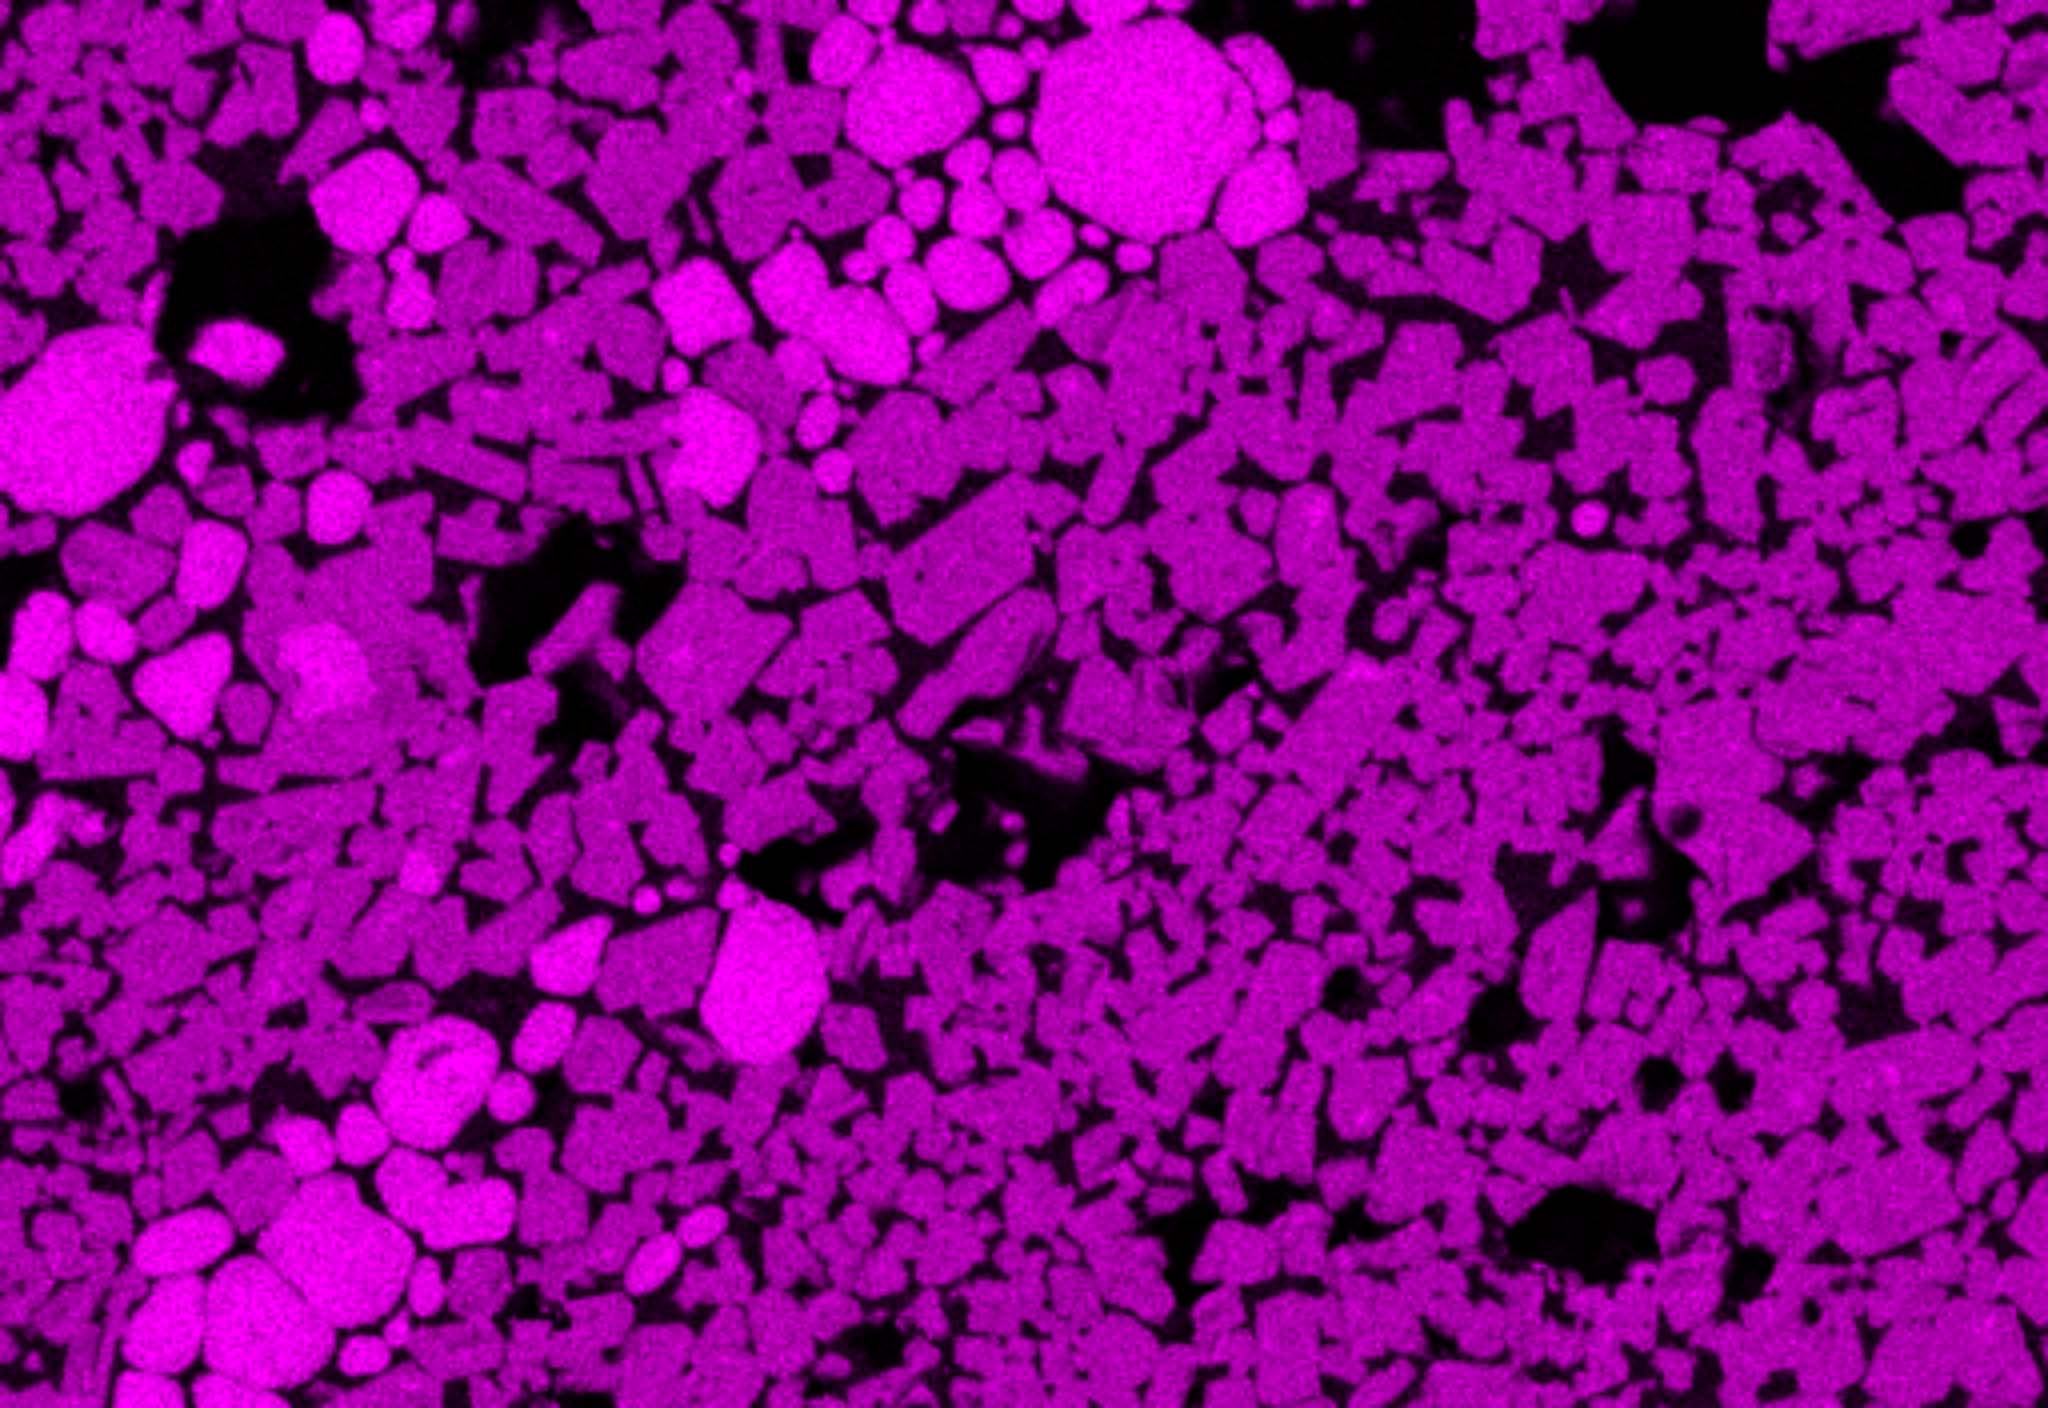
\includegraphics[width=\textwidth]{figures/la-icp-ms/edx/Si.jpg}
    \caption{Si mapping}
    \label{fig:LAICPMS-EDX-Si}
  \end{subfigure}
  \hfill
  \begin{subfigure}[t]{0.32\textwidth}
    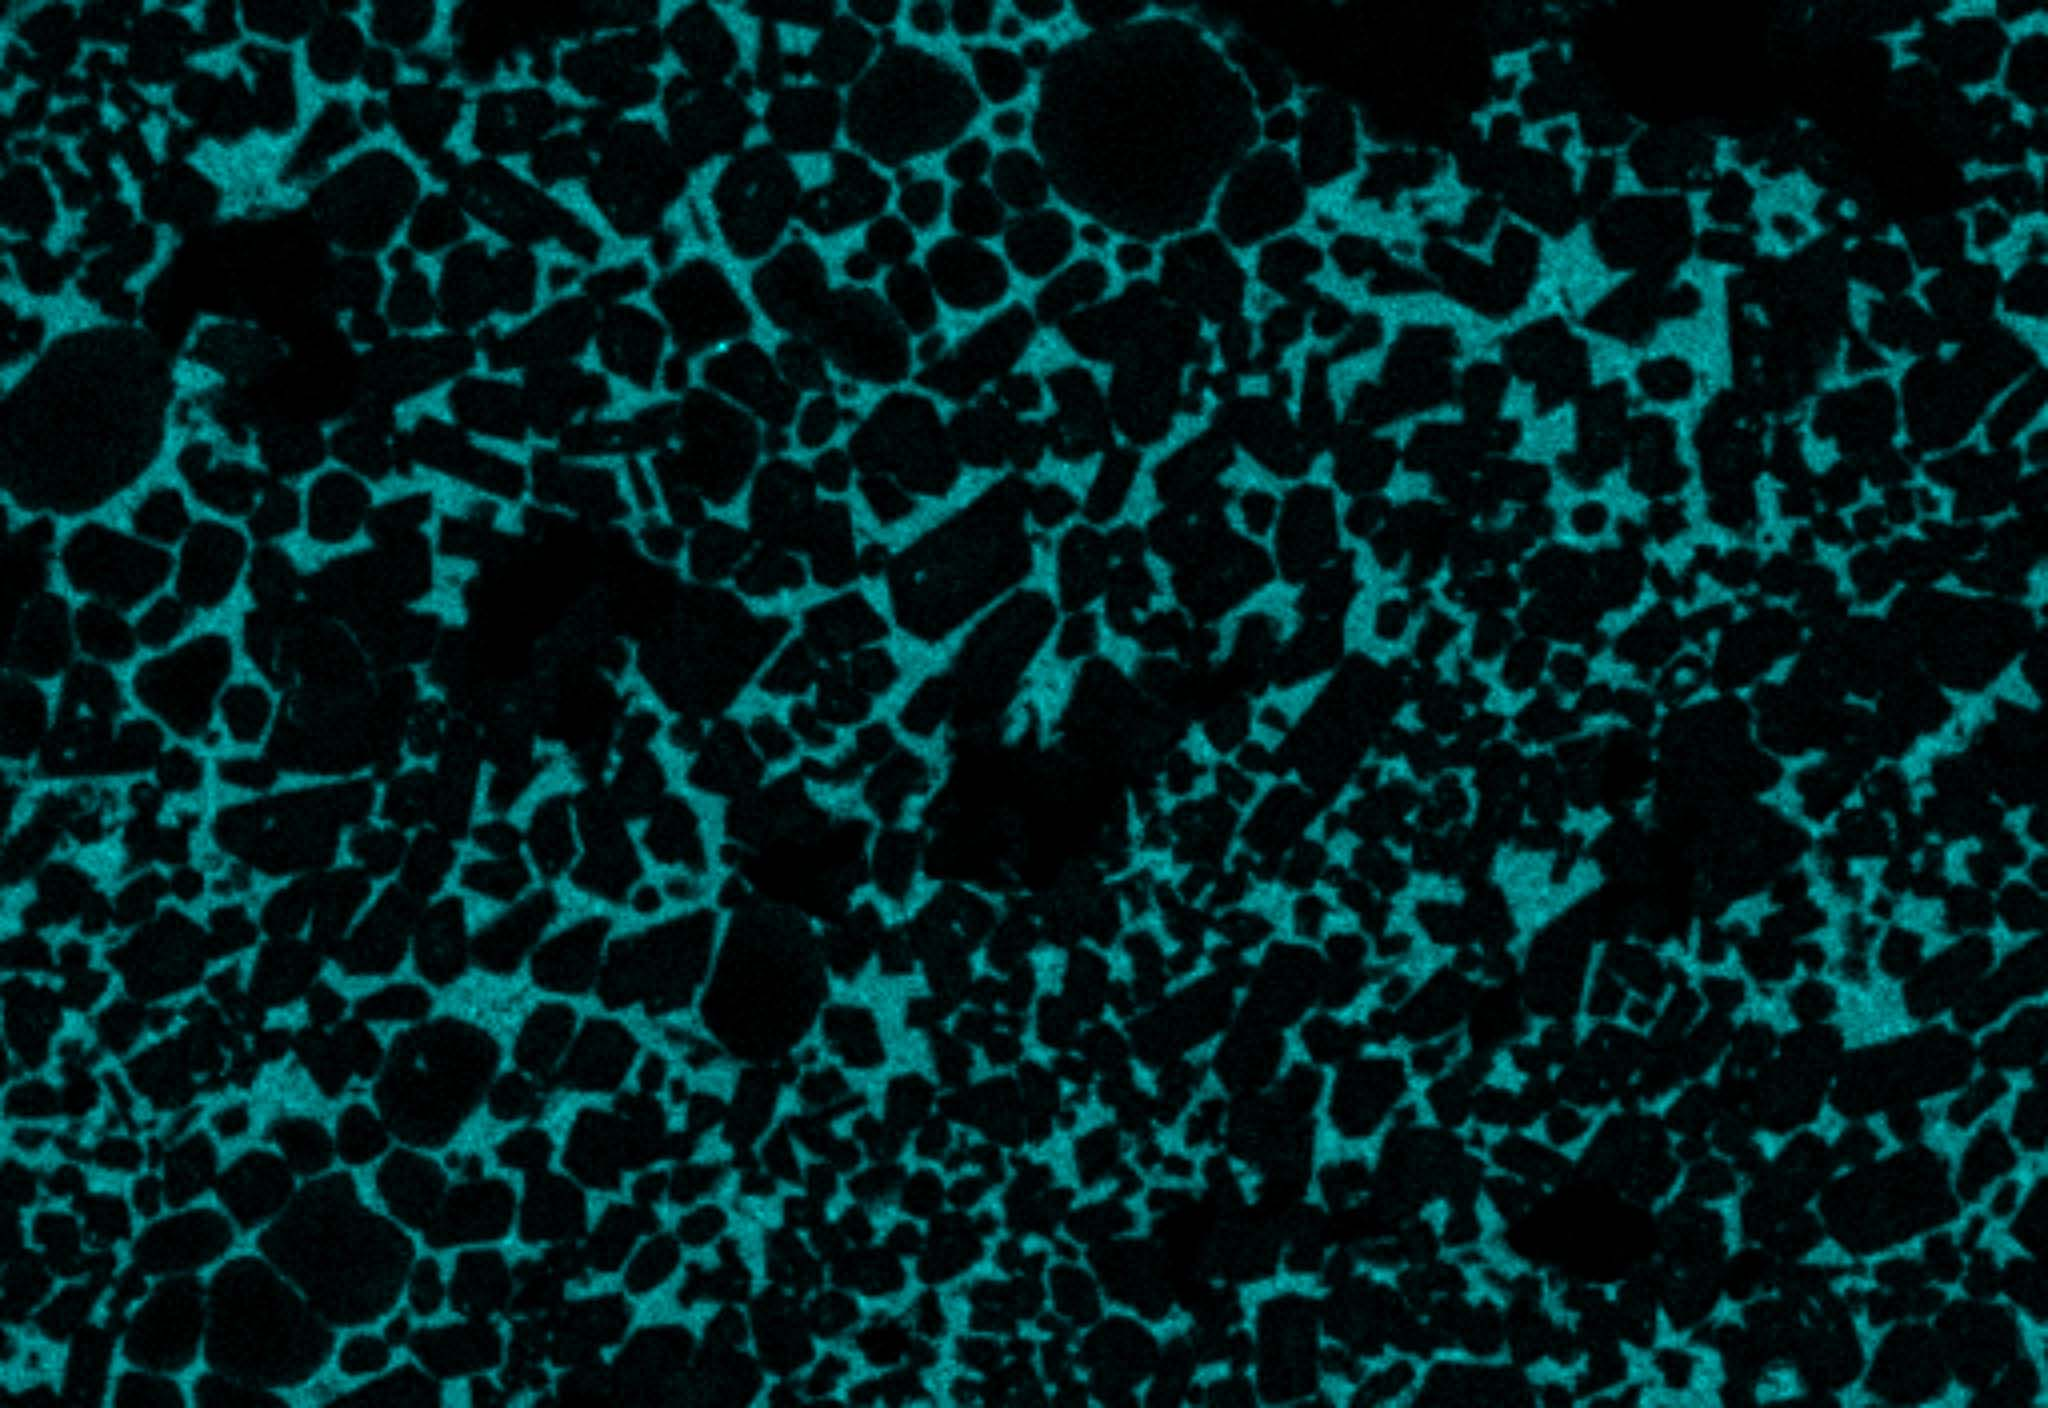
\includegraphics[width=\textwidth]{figures/la-icp-ms/edx/Al.jpg}
    \caption{Al mapping}
    \label{fig:LAICPMS-EDX-Al}
  \end{subfigure}

  \begin{subfigure}[t]{0.32\textwidth}
    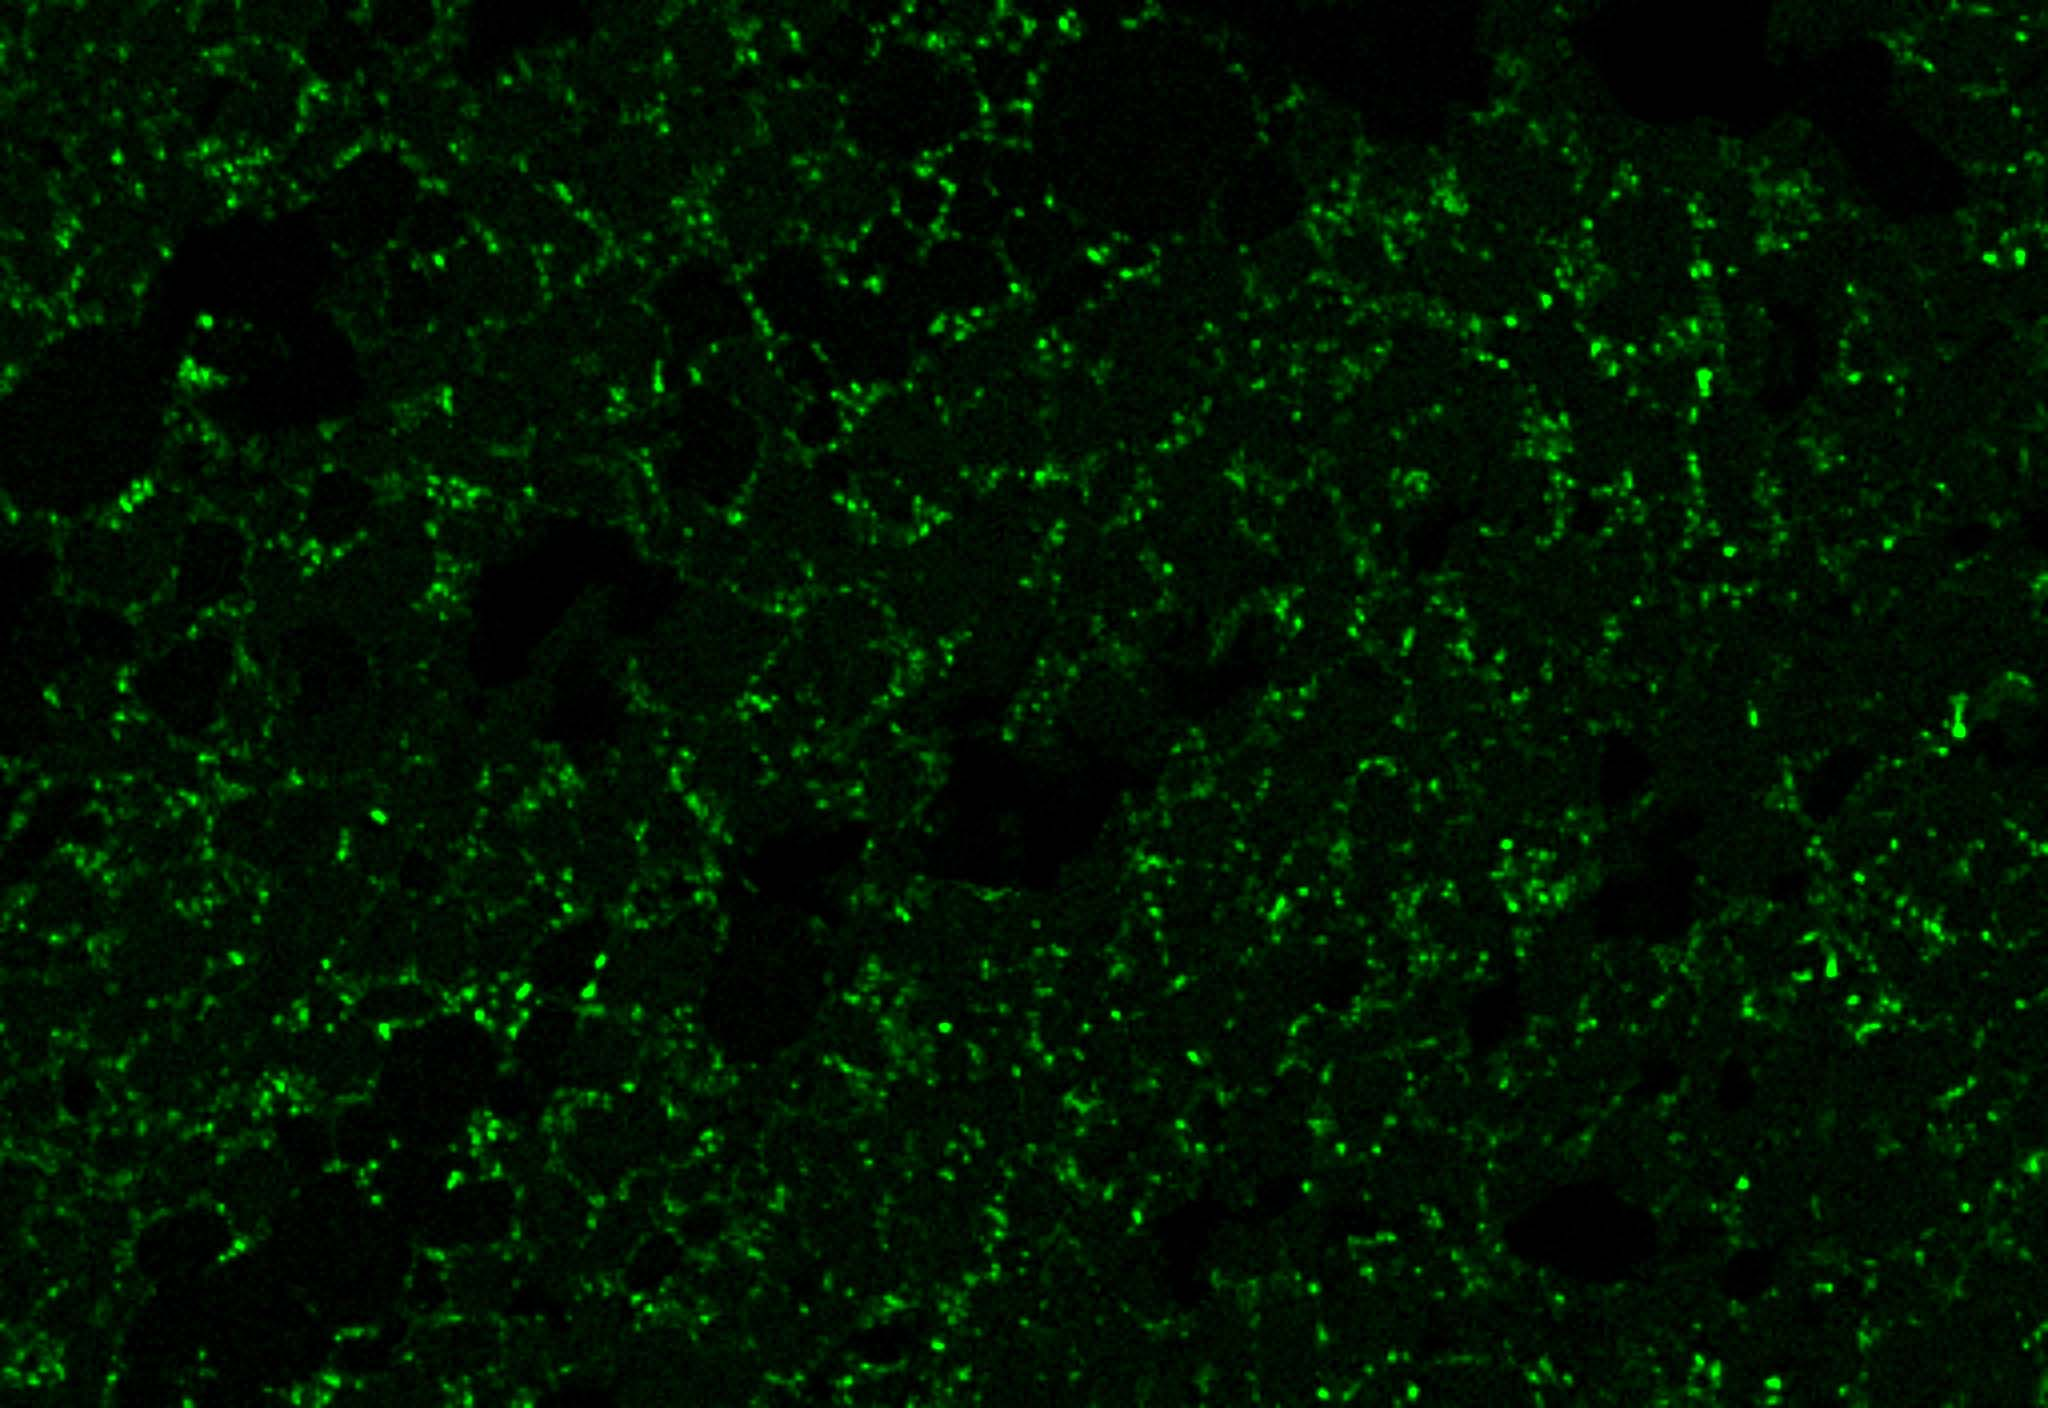
\includegraphics[width=\textwidth]{figures/la-icp-ms/edx/Mg.jpg}
    \caption{Mg mapping}
    \label{fig:LAICPMS-EDX-Mg}
  \end{subfigure}
  \hfill
  \begin{subfigure}[t]{0.32\textwidth}
    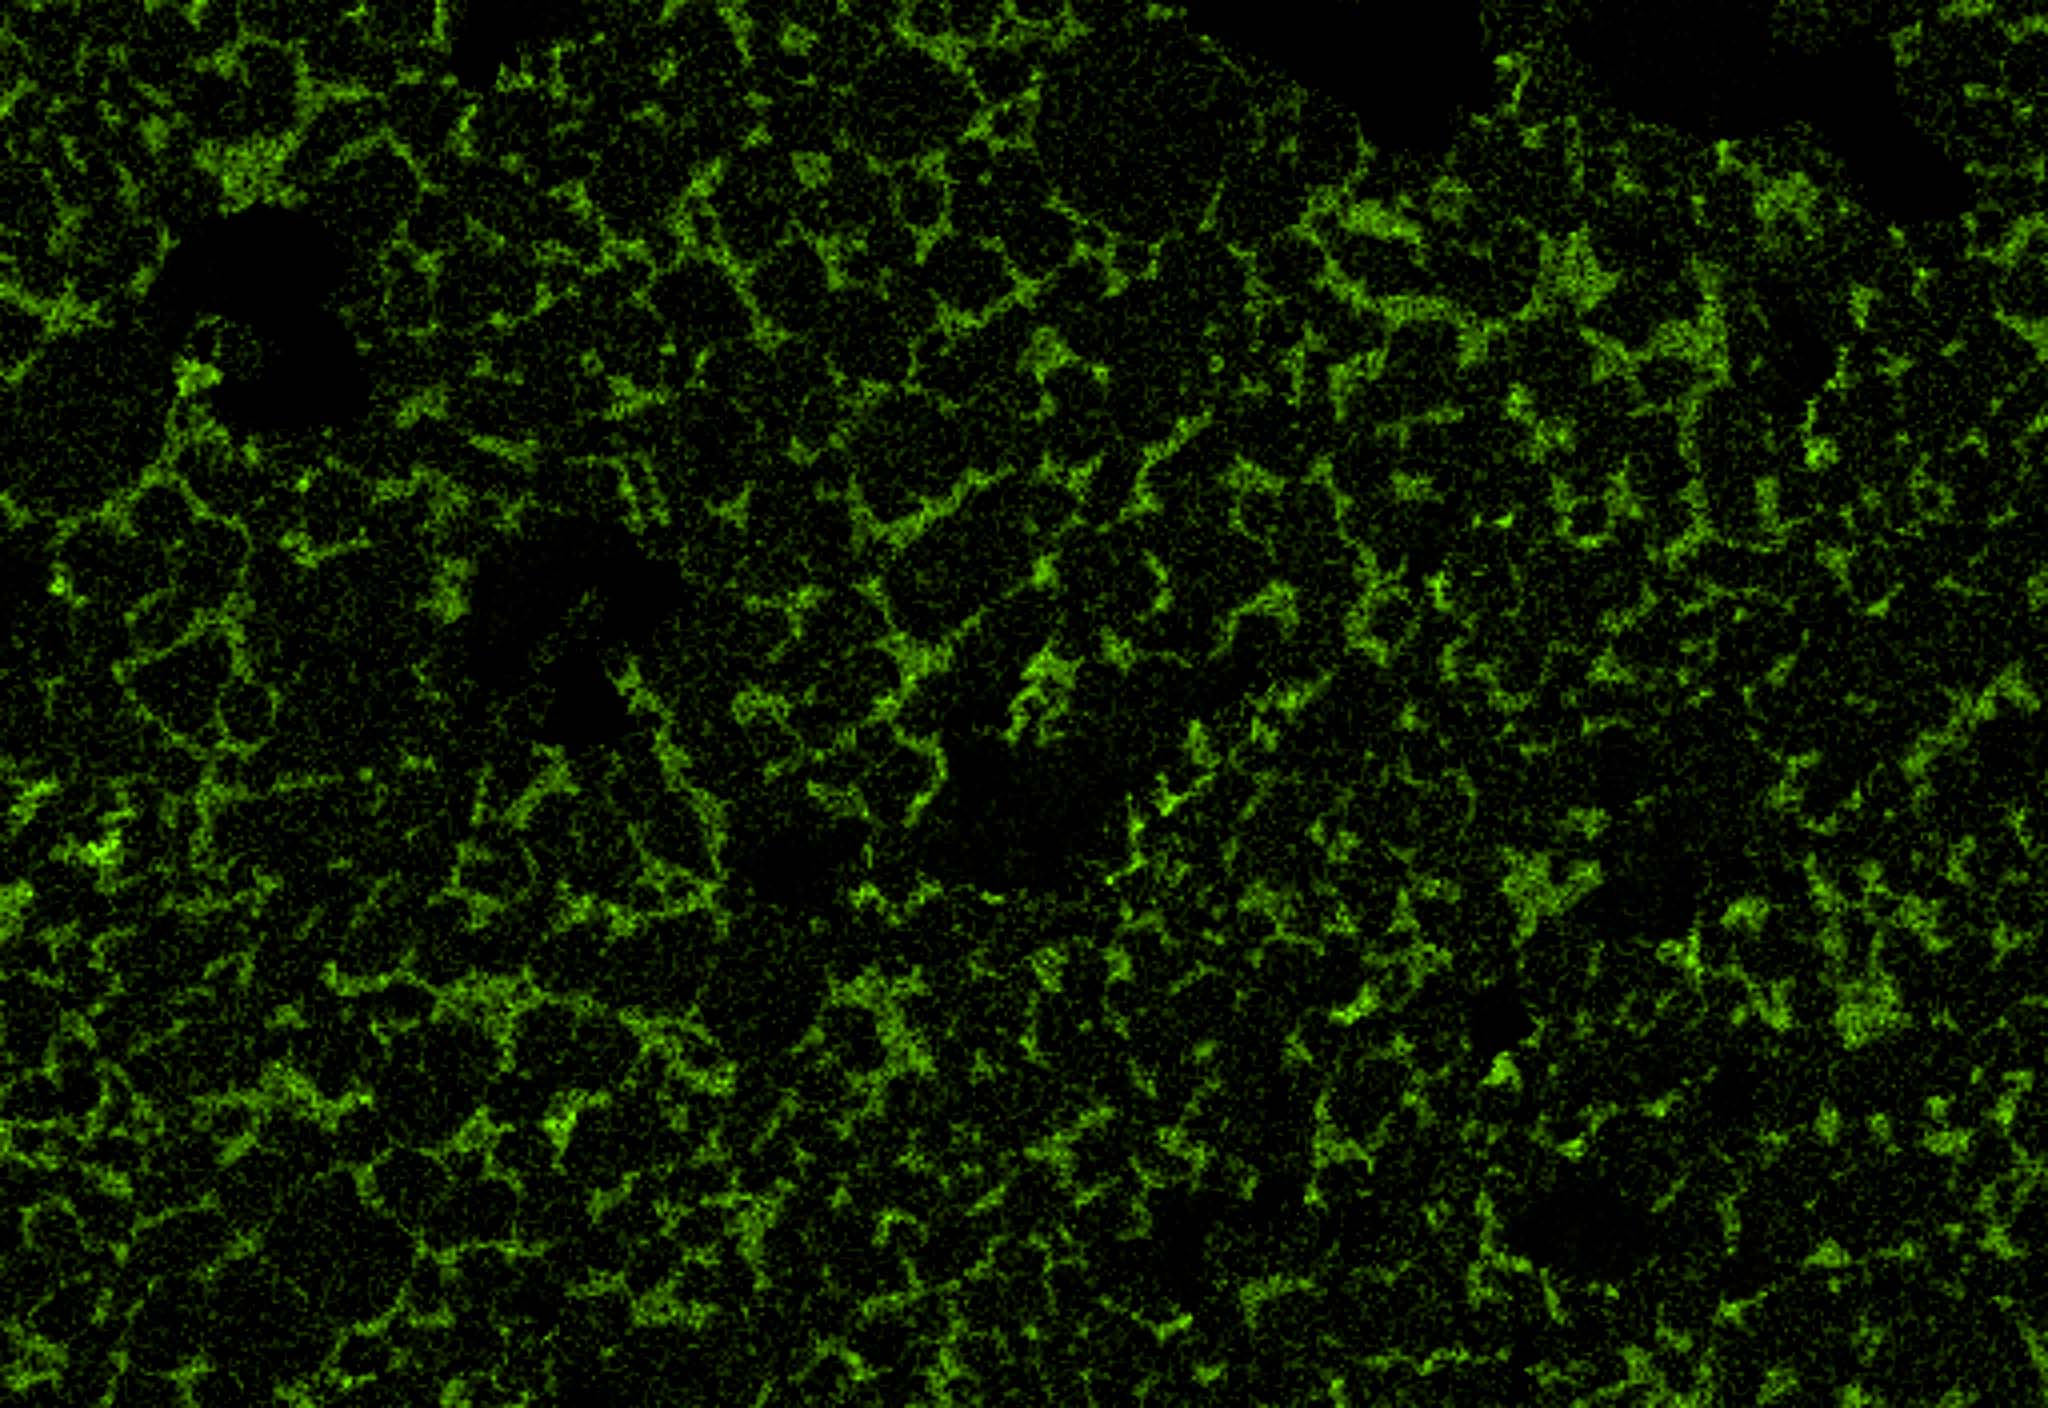
\includegraphics[width=\textwidth]{figures/la-icp-ms/edx/Fe.jpg}
    \caption{Fe mapping}
    \label{fig:LAICPMS-EDX-Fe}
  \end{subfigure}
  \hfill
  \begin{subfigure}[t]{0.32\textwidth}
    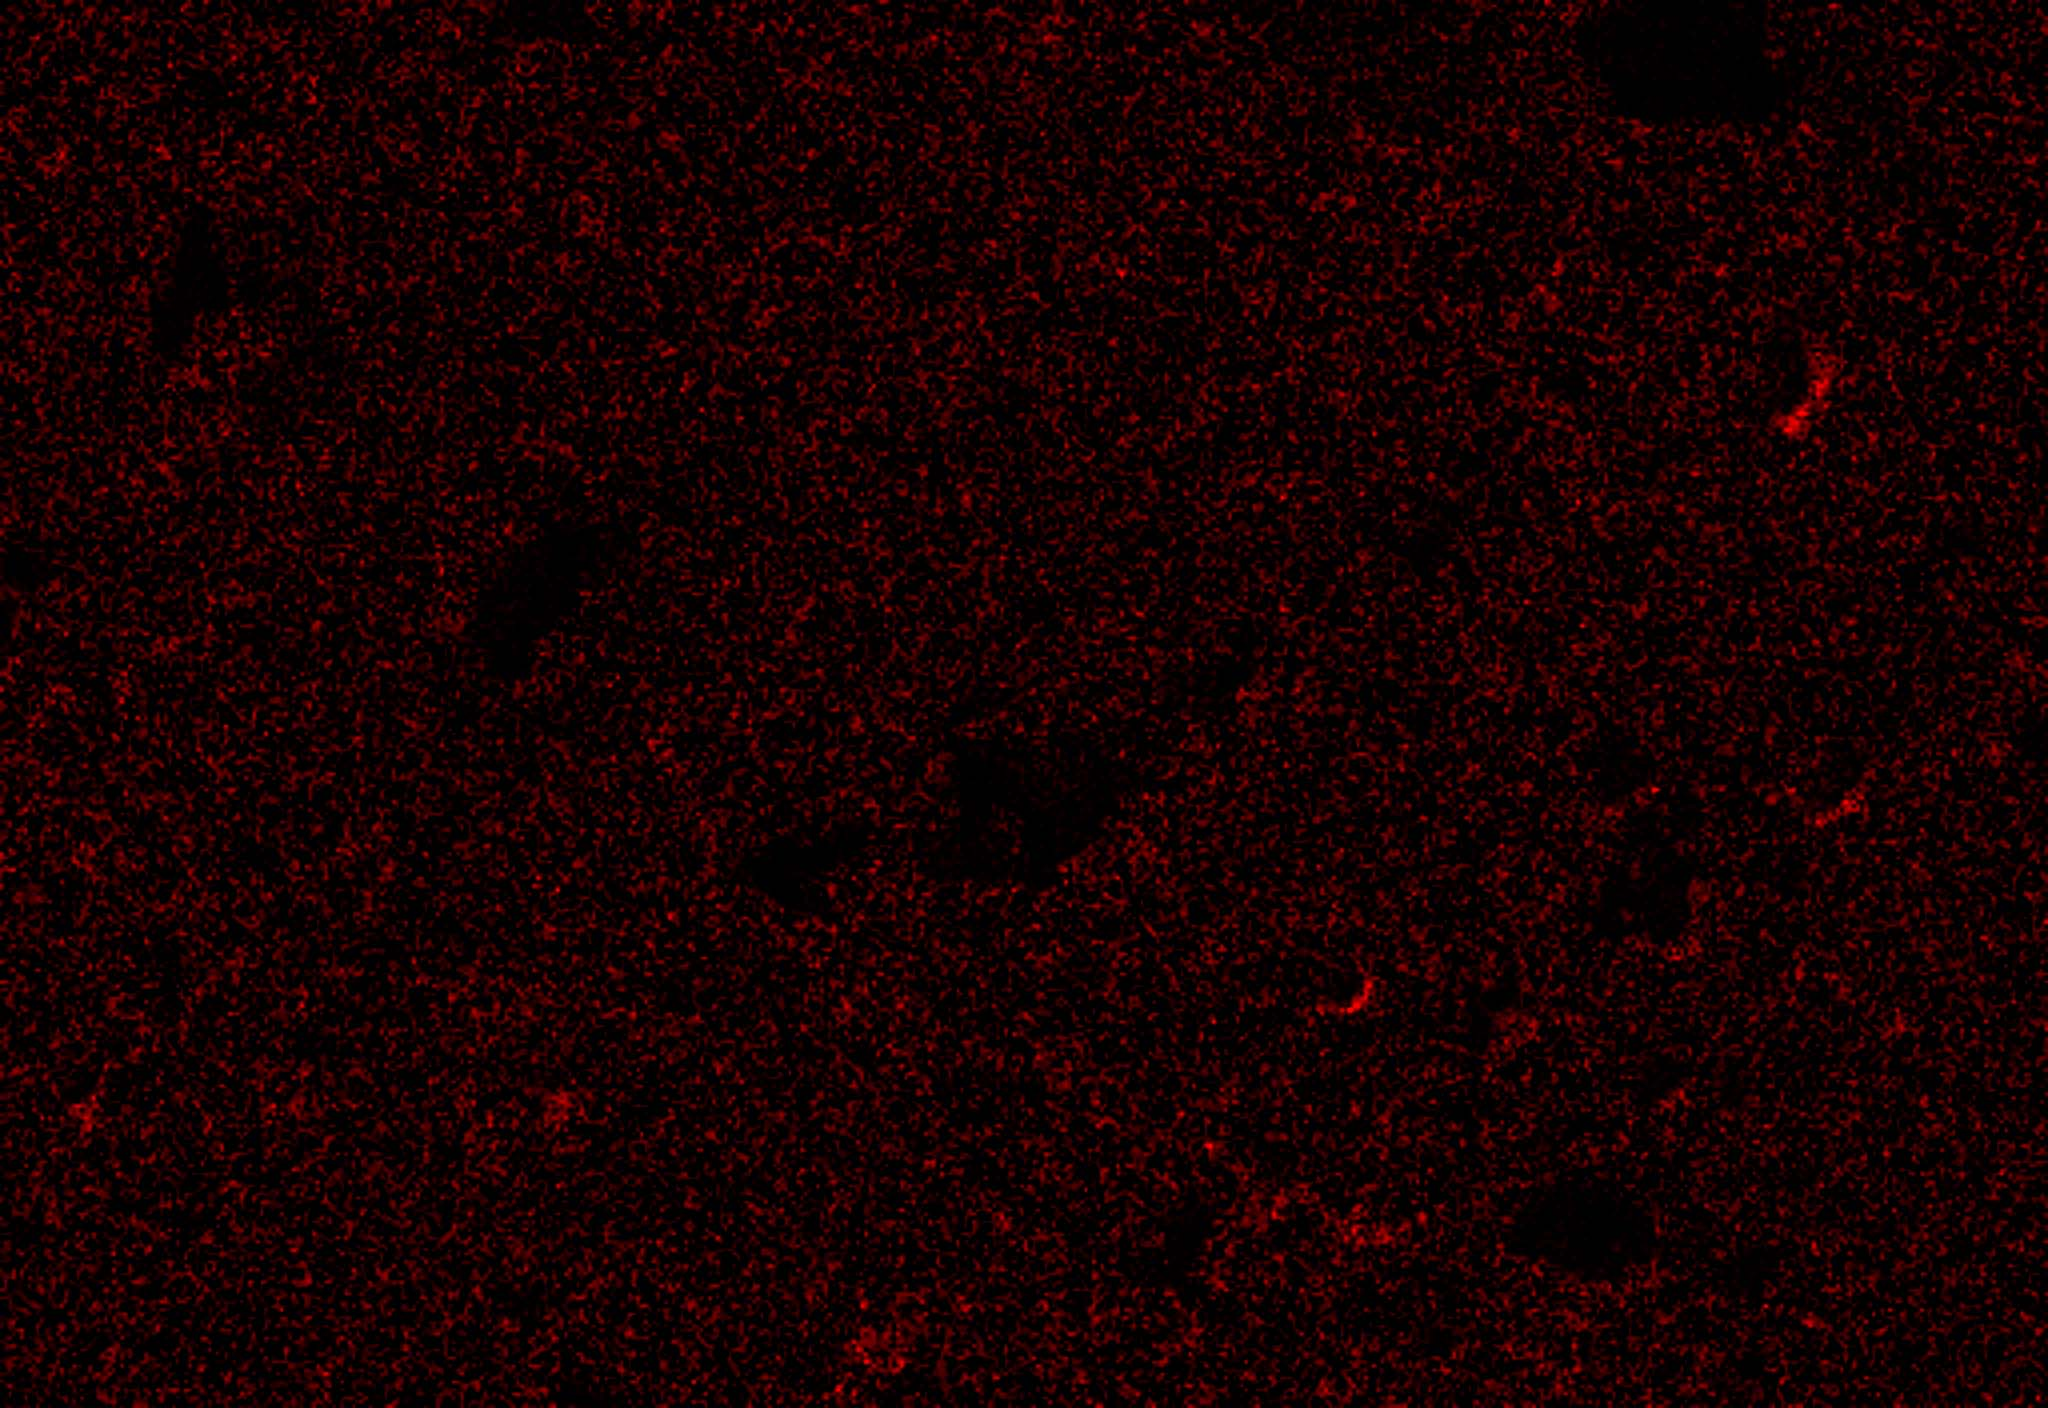
\includegraphics[width=\textwidth]{figures/la-icp-ms/edx/Na.jpg}
    \caption{Na mapping}
    \label{fig:LAICPMS-EDX-Na}
  \end{subfigure}

  \begin{subfigure}[t]{0.32\textwidth}
    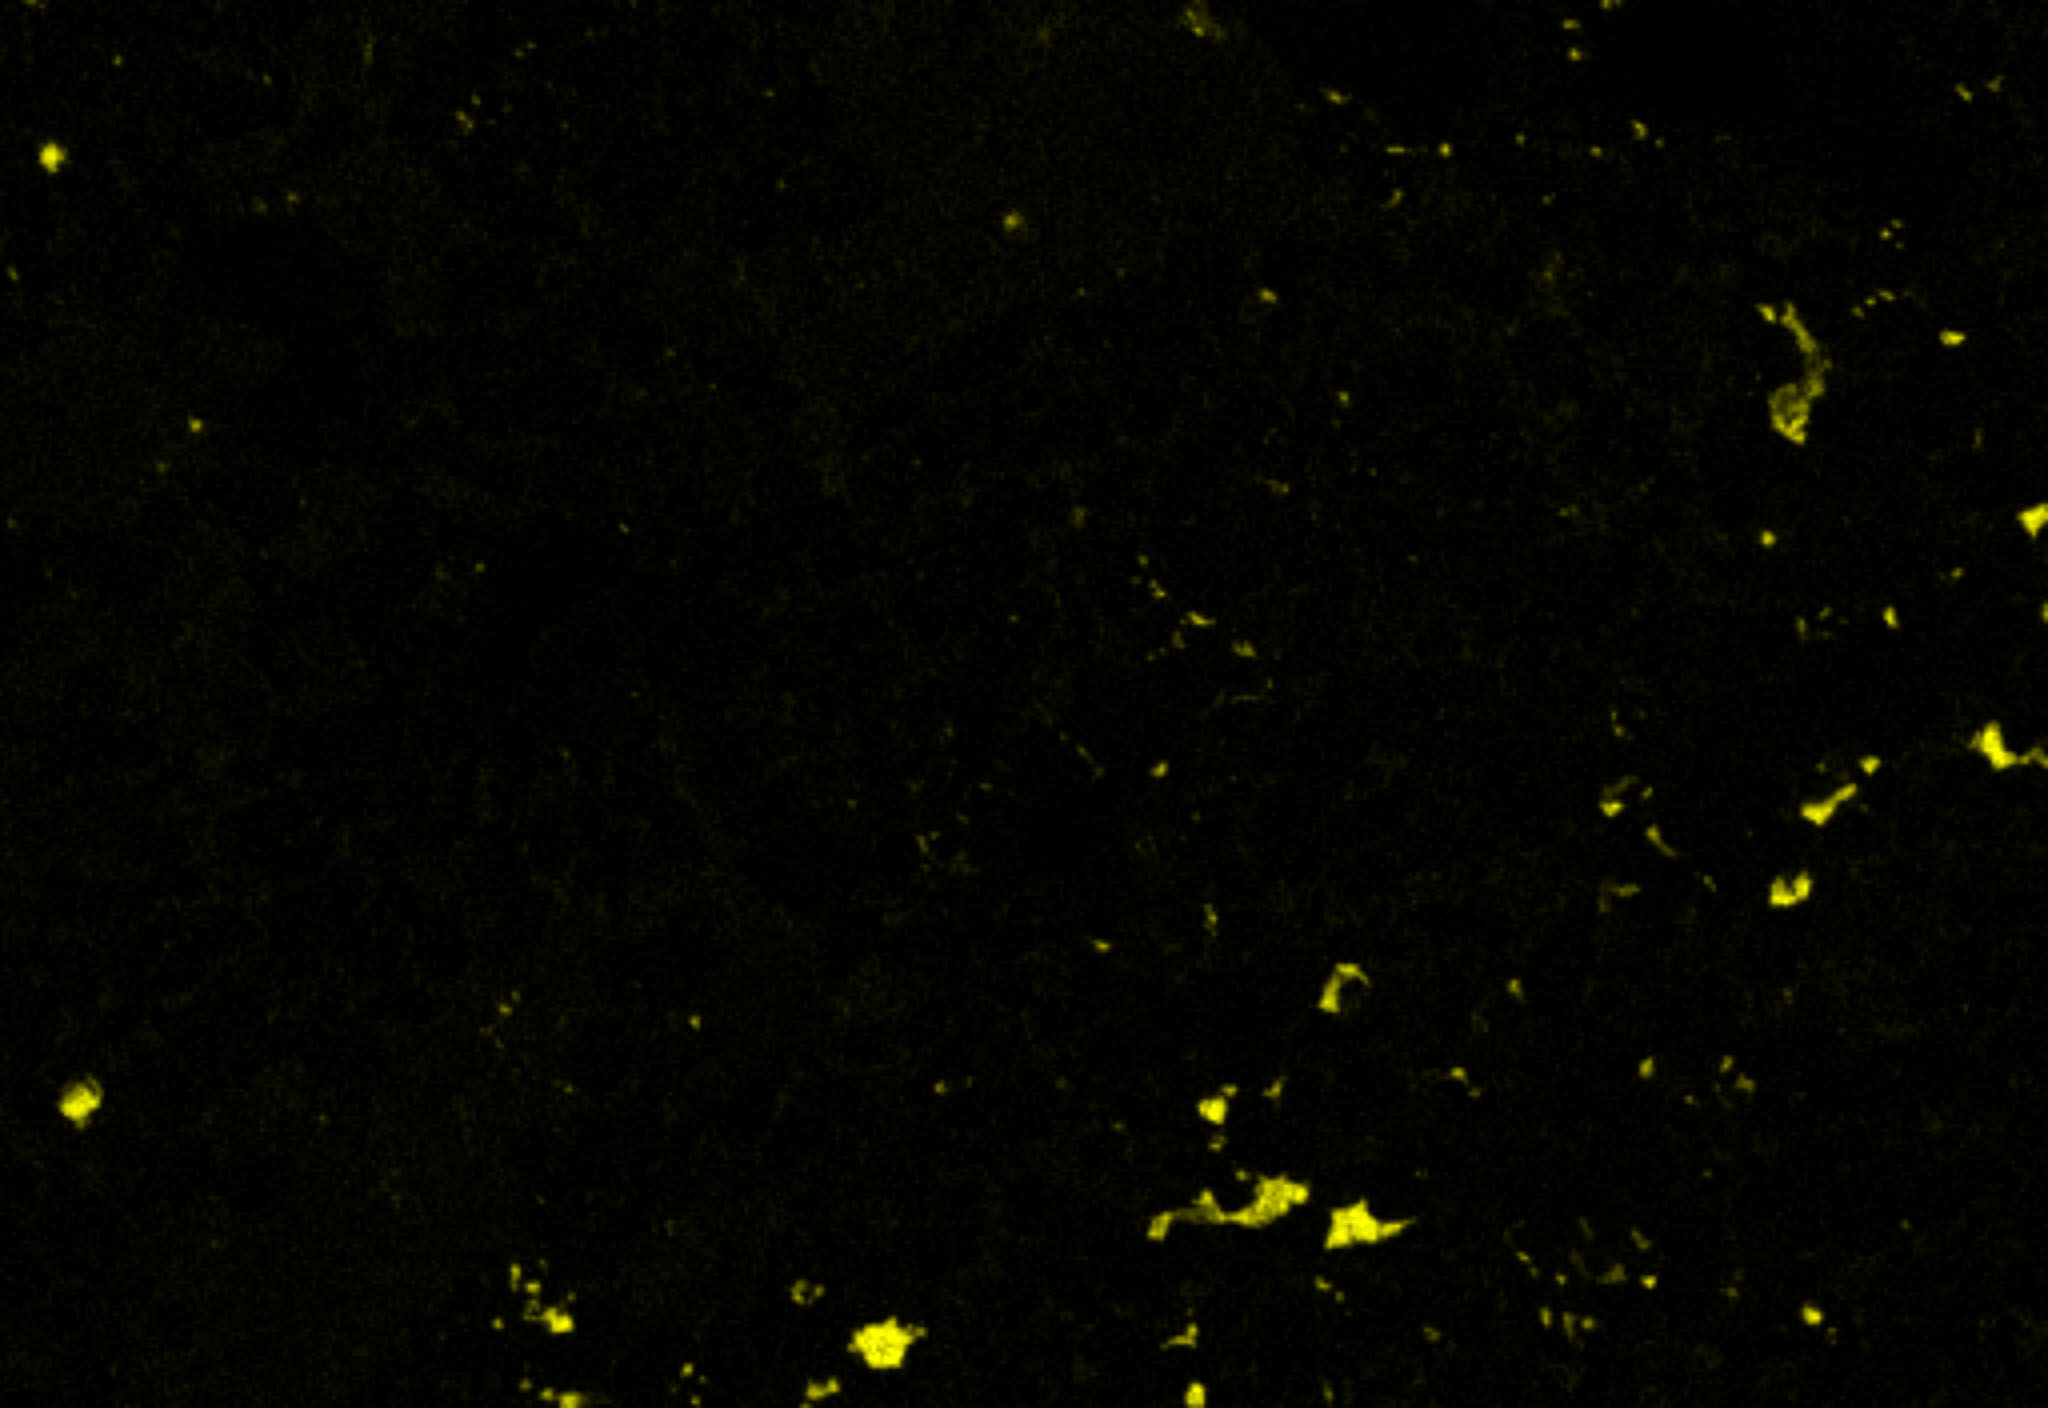
\includegraphics[width=\textwidth]{figures/la-icp-ms/edx/K.jpg}
    \caption{K mapping}
    \label{fig:LAICPMS-EDX-K}
  \end{subfigure}
  \hfill
  \begin{subfigure}[t]{0.32\textwidth}
    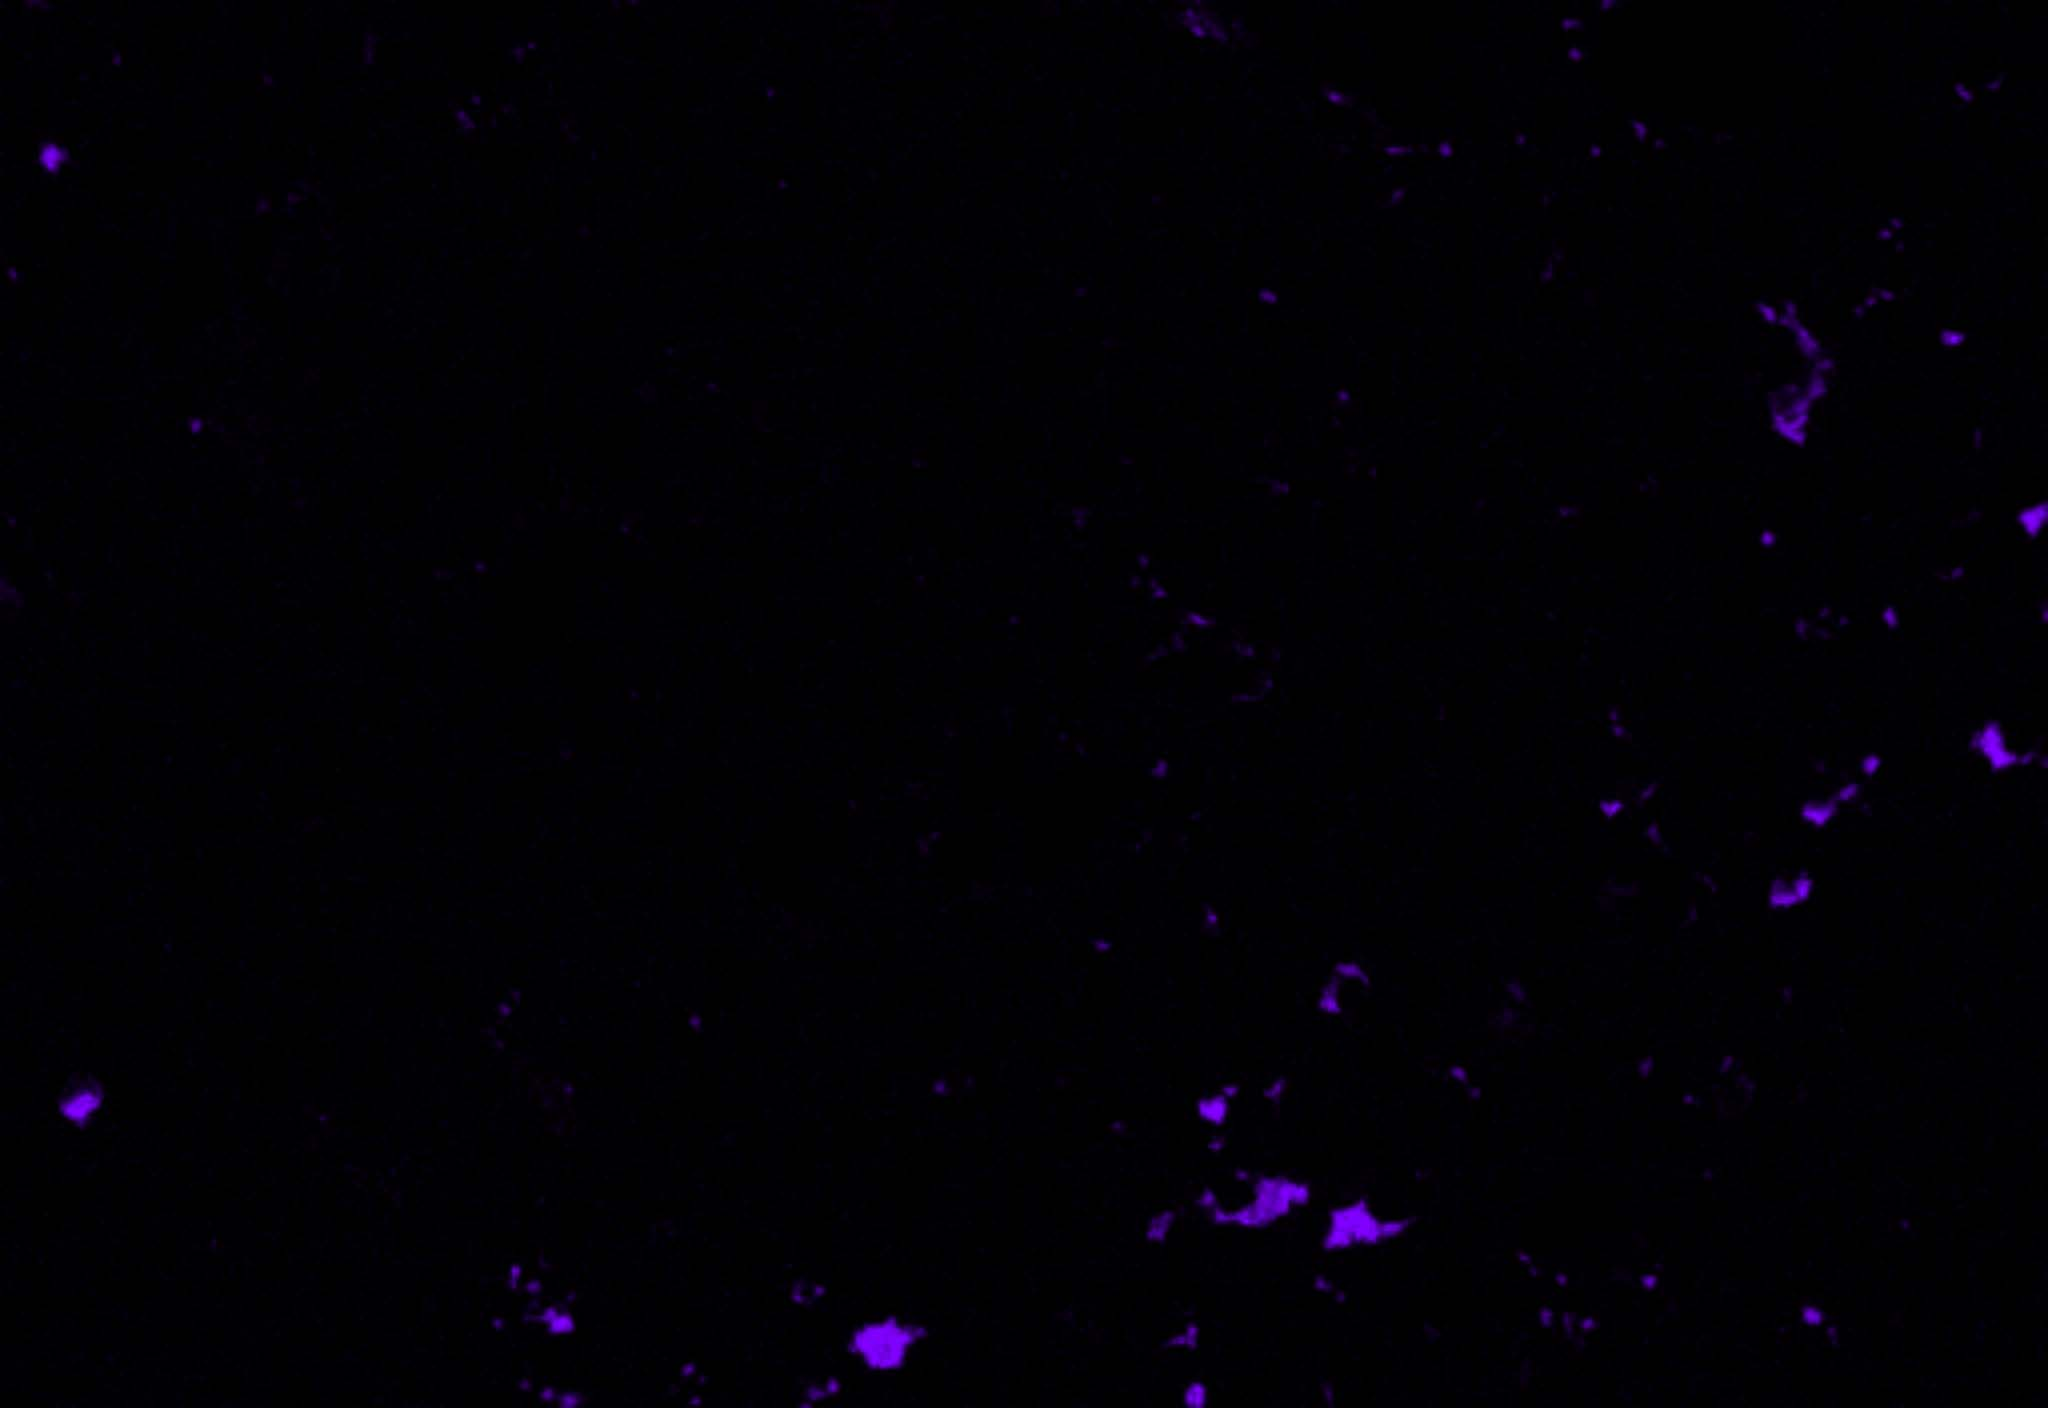
\includegraphics[width=\textwidth]{figures/la-icp-ms/edx/S.jpg}
    \caption{S mapping}
    \label{fig:LAICPMS-EDX-S}
  \end{subfigure}
  \hfill
  \begin{subfigure}[t]{0.32\textwidth}
    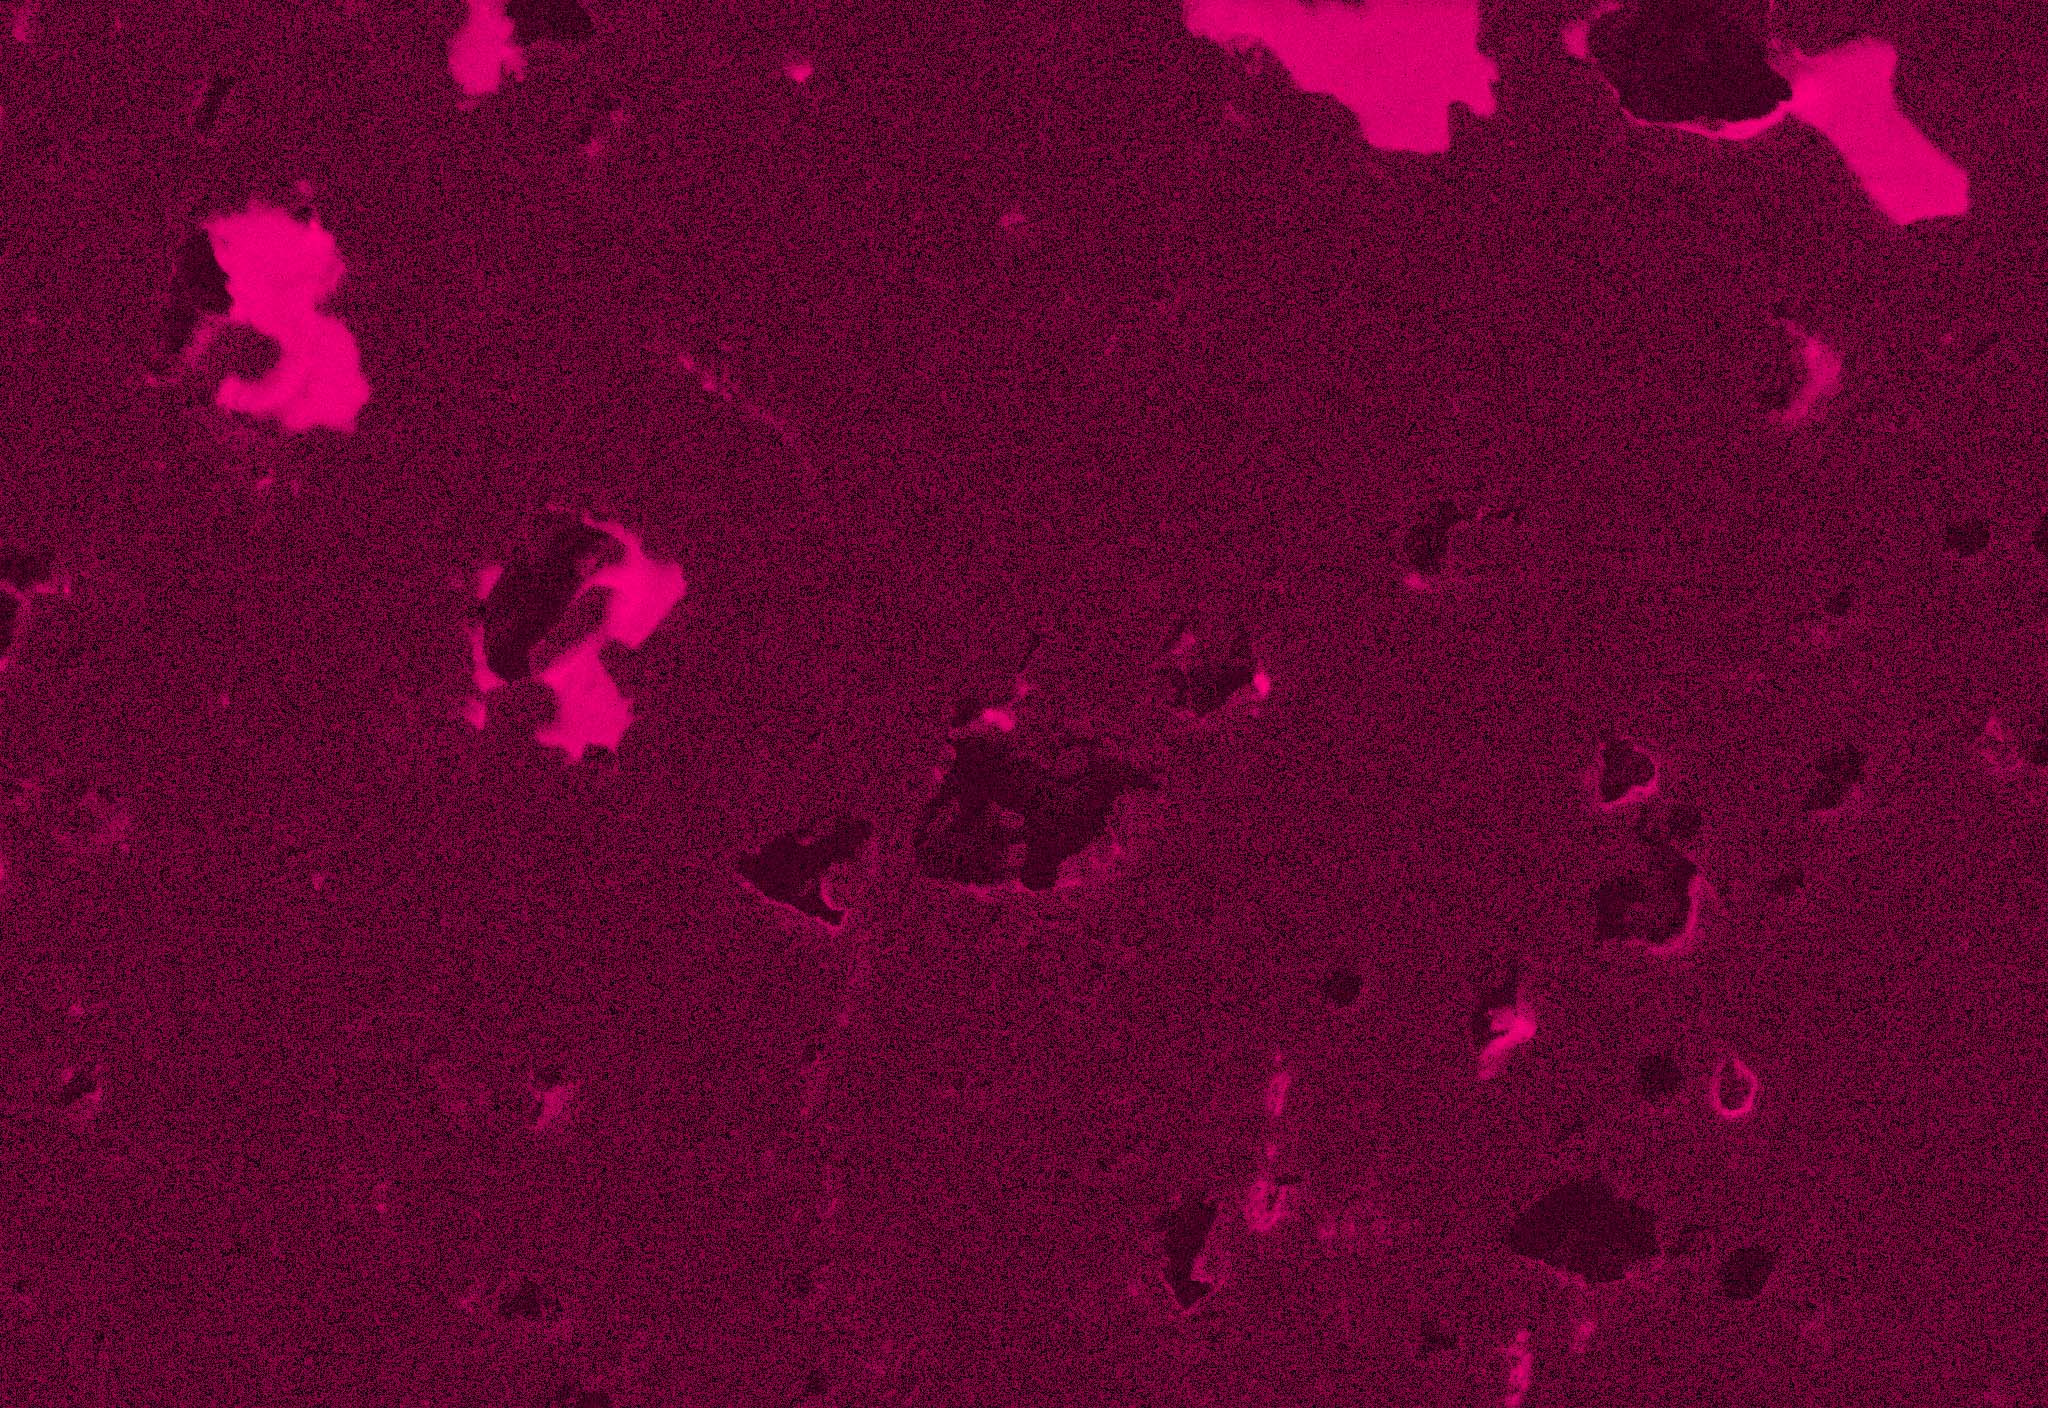
\includegraphics[width=\textwidth]{figures/la-icp-ms/edx/C.jpg}
    \caption{C mapping (epoxy resin)}
    \label{fig:LAICPMS-EDX-C}
  \end{subfigure}

  \caption{
    Element distribution maps of \ce{Ca}, \ce{Si}, \ce{Al}, \ce{Mg}, \ce{Fe}, \ce{Na}, \ce{K}, \ce{S}, and \ce{C}  of the example area.
    The maps have dimensions of \qtyproduct{414 x 285}{\micro\meter}.
    Data published in the \ac{SI} in \cite{kleiner.2022b}.
  }
  \label{fig:LAICPMS-EDX}
\end{figure}

A full phase map was calculated using the software \textit{Aztec 5.0} \cite{aztec.2004} and the result is shown in \zcref{fig:LAICPMS-phasemap}.
The comparison with the \ce{Si} element distribution map in \zcref{fig:LAICPMS-EDX-Si} reveals that the phase map distinguishes \ac{C3S}, \ac{C2S}, \ce{MgO}, and alkali sulphates quite well.
\ac{C3A} and \ac{C4AF} are difficult to differentiate within the \ac{LAICPMS} dataset and therefore, are combined and denoted as `interstitial phase' from here on (marked blue in \zcref{fig:LAICPMS-phasemap}).

%\begin{wrapfigure}{R}{0.6\linewidth}
\begin{figure}[htb!]
  \centering
  %\vspace{-\intextsep}
  \includegraphics[width=.9\linewidth]{la-icp-ms/EDX-phase-map.pdf}
  \caption{Phase map based on the \ac{EDX} dataset (see \zcref{fig:LAICPMS-EDX}). \cite{kleiner.2022b}, \ac{SI}}
  \label{fig:LAICPMS-phasemap}
  %\vspace{-\intextsep}
\end{figure}
%\end{wrapfigure}

\ac{C2S} can be seen mainly on the left half of the image in three clusters containing less \ce{Ca} and more \ce{Si} compared to \ac{C3S}.
The \ce{Al}-rich interstitial phases can best be seen in the \ac{EDX} mappings, while they usually appear as light (\ac{C4AF}) to medium grey (\ac{C3A}) in the \ac{BSE} image between the \ac{C3S} grains.

The positions of the minor phases \ce{K2SO4} and \ce{MgO} are indicated by the \ce{Mg} and \ce{S} distributions (\zcref{fig:LAICPMS-EDX-Mg} and \zcref{fig:LAICPMS-EDX-S}).
However, the location of \ce{MgO} is not visible in the phase map.
Elements like \ce{C} and \ce{Cl} cannot be considered for further analysis, since they are contained in the epoxy resin.
%In contrast, the maps of \ce{Na} and \ce{Ti} are very noisy and difficult to interpret.
%These mappings can be found in Figure~S-2.

%At least for unhydrated clinker, the individual phases seemed to be damaged in a similar fashion, while the epoxy resin was ablated a lot deeper.

The signal of other elements like \ce{Ti}, \ce{Cr}, \ce{Cu}, \ce{Mn} and \ce{P} was too low to generate useful element distribution maps.
Generally, elemental maps can be obtained in good quality if the X-ray count of the respective mappings is increased by increasing the measurement time.
However, the \ac{EDX} quality was not the major focus of this study.

\begin{figure}[!htb]
  \centering
  \begin{tikzpicture}
    \begin{semilogyaxis}[
        xtick = data,
        symbolic x coords={Ca,Si,Al,Fe,Mg,K,S,Na,Ti,P,Mn,Cr},
        table/col sep=comma,
        log origin=infty,
        width=\textwidth,
        height=7cm,
        ybar,
        bar width=8pt,
        enlarge x limits=0.07,
        ylabel={mass fraction in \unit{\wtpercent}},
        ytick={0.01,0.1,1,10,100},
        yticklabels={0.01,0.1,1,10,100},
        ymin=0.008, ymax=100,
        legend cell align=left,
        legend style={
            at={(0.98,0.97)},
            anchor=north east,
            column sep=4pt
        },
        legend columns=-1,
        error bars/y dir=both,
        error bars/y explicit,
        scaled y ticks = false,
        error bars/y dir=both,
        error bars/y explicit,
    ]

      \addplot[
        darkgreen,fill=darkgreen,
      ] table [
        x=element,
        y=c_analy_alt,
        col sep=comma
      ] {figures/la-icp-ms/chemical-edx.csv};
      \addlegendentry{\acs*{ICP}-\acs*{OES} analysis};

      \addplot[
        red, fill=red,
        error bars/.cd,
        error bar style={black},
      ] table [
        x=element,
        y=EDX_mean_area,
        y error=stabw_edx_area,
        col sep=comma
      ] {figures/la-icp-ms/chemical-edx.csv};
      \addlegendentry{\ac*{EDX} analysis};

      \draw [darkred, thick, dashed] (axis cs:Ca, 0.1) node [below, anchor=north west, align=left, text=black, fill=white, fill opacity=0.7, text opacity=1] {below the \ac{EDX} detection limit} -- (axis cs:Cr, 0.1) ;

    \end{semilogyaxis}
  \end{tikzpicture}
  \caption{
    Comparison of the results (oxide concentrations) from the chemical analysis (\ac{ICP}-\ac{OES}; see \zcref{tab:laicpms-clinker}) and the \ac{EDX} analysis obtained from the sum spectra of the three mappings.
    \cite{kleiner.2022b}
  }
  \label{fig:LAICPMS-EDX-chemical}
\end{figure}

To validate the \ac{EDX} results, the values were compared to the \ac{ICP}-\ac{OES} measurement (see \zcref{tab:laicpms-clinker}).
For this purpose, the \ac{EDX} results were averaged over the three mappings and the results were plotted in \zcref{fig:LAICPMS-EDX-chemical}.
However, the \ac{ICP}-\ac{OES} results are mostly within the range of the \ac{EDX} standard deviations.
The mass fraction of \ce{S} and \ce{Mg} and other low concentrated elements show obvious differences.
This indicates that the area analysed using \ac{EDX} is too small to be representative of the bulk composition, so that a chemical composition close to the \ac{ICP}-\ac{OES} results cannot be obtained.
While elements like \ce{Na}, \ce{P}, \ce{Mn}, and \ce{Cr} are detectable in the sum spectrum, their local concentrations within the mapping often fall below the practical \ac{EDX} detection limits.
Consequently, mass fractions below \qty{0.1}{\wtpercent} are treated as estimated values rather than absolute concentrations.
This concerns the elements \ce{Na}, \ce{P}, \ce{Mn}, and \ce{Cr}.

\begin{figure}[htb!]
  \centering

  \ifdefined\PRINTABLE
    \includegraphics[width=\textwidth]{la-icp-ms/la-icp-ms-mapping/result0.pdf}
  \else
    \animategraphics[loop,autoplay,width=\textwidth]{1}{la-icp-ms/la-icp-ms-mapping/result}{0}{2}
  \fi

  \caption{
    Element distribution maps generated by \ac{LAICPMS}.
    The images cover an area of \qtyproduct{483.8 x 343.4}{\micro\meter\squared} using \numproduct{80 x 603} measurements.
    The colorbars are normalised to the maximum mass fraction of each element (in \unit{\wtpercent} oxide).
    The outlines for \ac{C3S} (black) and \ac{C2S} (white) were derived from the \ac{EDX} phase map shown in \zcref{fig:LAICPMS-phasemap}. \ac{SI} in \cite{kleiner.2022b}
  }
  \label{fig:LAICPMS-la-maps}
\end{figure}

Results in \zcref{fig:LAICPMS-la-maps} show the element distribution maps obtained by \ac{LAICPMS}.
Some elements show regions of very high mass fractions, which will be called hotspots henceforth.
A comparison of the \ce{Al} element distribution maps obtained by both methods (\zcref{fig:LAICPMS-EDX, fig:LAICPMS-la-maps}) reveals that \ac{LAICPMS} does not distinctly resolve the phase boundaries between the finely grained interstitial phases (\ac{C3A} and \ac{C4AF}) and the silicate phases.
This limitation becomes particularly apparent when the size of the laser ablation spot exceeds that of the individual phases, such as \ac{C3A} and \ac{C4AF}.
By combining phase segmentation based on the \ac{EDX} maps with the \ac{LAICPMS} data (\zcref{fig:LAICPMS-la-maps}), the relevant phases (\ac{C3S}, \ac{C2S}, \ac{C4AF}, and \ac{C3A}) can be analysed in detail.
A comparison of the quantification results obtained by \ac{EDX} and \ac{LAICPMS} for the interstitial phase is presented in \zcref{fig:LAICPMS-la-maps, fig:LA-EDX-results-high, fig:LA-EDX-results-low}.

The \ce{Al} content measured by \ac{EDX} and \ac{LAICPMS} at identical locations exhibits considerable variation (\zcref{fig:LA-EDX-results-low}).
For example, \ac{EDX} yielded a mass fraction of \qty{23.1}{\wtpercent}, whereas \ac{LAICPMS} yielded \qty{7.8(4.2)}{\wtpercent}.
The observed discrepancy may be attributed to several factors, including potential inaccuracies in dataset alignment, calibration errors, and, most plausibly, phase heterogeneity caused by differences in the depth of the signal origin.
Nevertheless, the mass fraction determined for \ce{Al}, \ce{Mg}, \ce{Ti}, \ce{K}, \ce{Na}, and \ce{Mn} (\zcref{fig:LA-EDX-results-high, fig:LA-EDX-results-low}) consistently remain within the same order of magnitude.
These findings prove that the laser spot size (\qtyproduct{6x6}{\micro\meter\squared}) is too large to quantitatively analyse the interstitial phases.
Nevertheless, enrichment of, for example, \ce{Mn} in the interstitial phase can be demonstrated by \ac{LAICPMS}.
Furthermore, an inaccurate image registration seems to be a minor problem, as the same trends in major, minor and trace element concentration can be found in all investigated areas (cf. \zcref{tab:laicpms1-area1, tab:laicpms2-area1,tab:laicpms1-area2, tab:laicpms2-area2,tab:laicpms1-area3, tab:laicpms2-area3}, as in the \ac{SI} from \cite{kleiner.2022b}).

\begin{figure}[!htb]
  \centering

  % Subfigure 1: Alite
  \begin{subfigure}[b]{0.36\textwidth}
    \begin{tikzpicture}
      \begin{semilogyaxis}[
          xtick=data,
          symbolic x coords={Al,Mg,K,Na,Ti},
          ytick={0.001,0.01,0.1,1,10},
          yticklabels={0.001,0.01,0.1,1,10},
          xticklabel style={font=\footnotesize},
          yticklabel style={font=\footnotesize},
          table/col sep=comma,
          width=1.05\textwidth,
          height=6cm,
          log origin=infty,
          ybar,
          bar width=5pt,
          enlarge x limits=0.15,
          ylabel={mass fraction in \unit{\percent}},
          ymin=0.008, ymax=40,
          error bars/y dir=both,
          error bars/y explicit,
          scaled y ticks = false,
      ]
        \addplot[
          cyan,fill=cyan,
          error bars/.cd,
          error bar style={black},
        ] table [
          x=Isotope,
          y=La_map_c_C3S,
          y error=La_map_err_C3S,
          col sep=comma
        ] {figures/la-icp-ms/element_analysis_EDX_La.csv};

        \addplot[
          red,fill=red,
          error bars/.cd,
          error bar style={black},
        ] table [
          x=Isotope,
          y=EDX_map_c_C3S,
          y error=EDX_map_err_C3S,
          col sep=comma
        ] {figures/la-icp-ms/element_analysis_EDX_La.csv};

        \draw [darkred, thick, dashed] (axis cs:Al, 0.1) -- (axis cs:Ti, 0.1);
        \node[above, font=\footnotesize, xshift=-4pt] at (axis cs:K, 2) {*};

      \end{semilogyaxis}
    \end{tikzpicture}
    \caption{\ac{C3S}}
    \label{fig:LA-EDX-results-alite}
  \end{subfigure}
  \hfill
  % Subfigure 2: Belite
  \begin{subfigure}[b]{0.30\textwidth}
    \begin{tikzpicture}
      \begin{semilogyaxis}[
          xtick=data,
          symbolic x coords={Al,Mg,K,Na,Ti},
          ytick={0.001,0.01,0.1,1,10},
          yticklabels={}, % Remove y tick labels
          xticklabel style={font=\footnotesize},
          table/col sep=comma,
          width=1.27\textwidth,
          height=6cm,
          log origin=infty,
          ybar,
          bar width=5pt,
          enlarge x limits=0.15,
          ylabel={}, % Remove y label
          ymin=0.008, ymax=40,
          legend cell align=center,
          legend style={
              at={(0.5,0.99)},
              anchor=north,
              column sep=4pt,
              font=\footnotesize
          },
          legend columns=-1,
          error bars/y dir=both,
          error bars/y explicit,
          scaled y ticks = false,
      ]
        \addplot[
          cyan,fill=cyan,
          error bars/.cd,
          error bar style={black},
        ] table [
          x=Isotope,
          y=La_map_c_C2S,
          y error=La_map_err_C2S,
          col sep=comma
        ] {figures/la-icp-ms/element_analysis_EDX_La.csv};
        \addlegendentry{\ac{LAICPMS}};

        \addplot[
          red,fill=red,
          error bars/.cd,
          error bar style={black},
        ] table [
          x=Isotope,
          y=EDX_map_c_C2S,
          y error=EDX_map_err_C2S,
          col sep=comma
        ] {figures/la-icp-ms/element_analysis_EDX_La.csv};
        \addlegendentry{\ac{EDX}};

        \draw [darkred, thick, dashed] (axis cs:Al, 0.1) -- (axis cs:Ti, 0.1);

      \end{semilogyaxis}
    \end{tikzpicture}
    \caption{\ac{C2S}}
    \label{fig:LA-EDX-results-belite}
  \end{subfigure}
  \hfill
  % Subfigure 3: C4AF
  \begin{subfigure}[b]{0.30\textwidth}
    \begin{tikzpicture}
      \begin{semilogyaxis}[
          xtick=data,
          symbolic x coords={Al,Mg,K,Na,Ti},
          ytick={0.001,0.01,0.1,1,10},
          yticklabels={},%{0.001,0.01,0.1,1,10},
          xticklabel style={font=\footnotesize},
          table/col sep=comma,
          width=1.27\textwidth,
          height=6cm,
          log origin=infty,
          ybar,
          bar width=5pt,
          enlarge x limits=0.15,
          ylabel={},%{Difference to mean concentration in \unit{\percent}},
          ymin=0.008, ymax=40,
          error bars/y dir=both,
          error bars/y explicit,
          scaled y ticks = false,
          yticklabel pos=right,
      ]
        \addplot[
          cyan,fill=cyan,
          error bars/.cd,
          error bar style={black},
        ] table [
          x=Isotope,
          y=La_map_c_C4AF,
          y error=La_map_err_C4AF,
          col sep=comma
        ] {figures/la-icp-ms/element_analysis_EDX_La.csv};

        \addplot[
          red,fill=red,
          error bars/.cd,
          error bar style={black},
        ] table [
          x=Isotope,
          y=EDX_map_c_C4AF,
          y error=EDX_map_err_C4AF,
          col sep=comma
        ] {figures/la-icp-ms/element_analysis_EDX_La.csv};

        \draw [darkred, thick, dashed] (axis cs:Al, 0.1) -- (axis cs:Ti, 0.1);
        \node[above, font=\footnotesize, xshift=-4pt] at (axis cs:K, 2) {*};

      \end{semilogyaxis}
    \end{tikzpicture}
    \caption{interstitial phase}
    \label{fig:LA-EDX-results-C4AF}
  \end{subfigure}

  \caption{
    Mean main element mass fraction for \ac{C3S}, \ac{C2S} and the interstitial phase, determined by segmented \ac{LAICPMS} mappings.
    Mass fractions below \qty{0.1}{\wtpercent} (marked as dashed line) are considered semi-quantitative, as the signal-to-noise ratio in the mapping data limits precise quantification in this range.
    Bars marked with an asterisk (*) have error bars extending beyond the axis range; only the upper limit is shown.
    Based on \cite{kleiner.2022b}
  }
  \label{fig:LA-EDX-results-high}
\end{figure}

%\begin{wrapfigure}{R}{0.6\linewidth}
\begin{figure}[!htb]
  \centering
  \begin{tikzpicture}
    \begin{semilogyaxis}[
        xtick=data,
        symbolic x coords={Mn,Zn,Ba,Cr,V,Rb},
        ytick={0.001,0.01,0.1,1},
        yticklabels={0.001,0.01,0.1,1},
        xticklabel style={font=\footnotesize},
        yticklabel style={font=\footnotesize},
        table/col sep=comma,
        width=.7\linewidth,
        height=6cm,
        log origin=infty,
        ybar,
        bar width=7pt,
        enlarge x limits=0.15,
        ylabel={concentration in \unit{\percent}},
        ymin=0.001, ymax=.3,
        error bars/y dir=both,
        error bars/y explicit,
        scaled y ticks = false,
        legend cell align=left,
        legend columns = 1,
        legend style={
            at={(1.03,0.5)},
            anchor=west,
            column sep=4pt
        },
    ]
    \addplot[
      orange,fill=orange,
      error bars/.cd,
      error bar style={black},
    ] table [
      x=Isotope,
      y=La_map_c_C3S,
      y error=La_map_err_C3S,
      col sep=comma
    ] {figures/la-icp-ms/element_analysis_LA.csv};

    \addplot[
      red,fill=red,
      error bars/.cd,
      error bar style={black},
    ] table [
      x=Isotope,
      y=La_map_c_C2S,
      y error=La_map_err_C2S,
      col sep=comma
    ] {figures/la-icp-ms/element_analysis_LA.csv};

    \addplot[
      blue,fill=blue,
      error bars/.cd,
      error bar style={black},
    ] table [
      x=Isotope,
      y=La_map_c_C4AF,
      y error=La_map_err_C4AF,
      col sep=comma
    ] {figures/la-icp-ms/element_analysis_LA.csv};

    \addlegendentry{\ac{C3S}};
    \addlegendentry{\ac{C2S}};
    \addlegendentry{interstitial phase};


    \node[above, font=\footnotesize, xshift=-9pt] at (axis cs:Zn, 0.08) {*};
    \node[above, font=\footnotesize] at (axis cs:Zn, 0.075) {*};
    \node[above, font=\footnotesize, xshift=+9pt] at (axis cs:Zn, 0.08) {*};

    \node[above, font=\footnotesize, xshift=-9pt] at (axis cs:Ba, 0.05) {*};
    \node[above, font=\footnotesize, xshift=+9pt] at (axis cs:Ba, 0.05) {*};

    \node[above, font=\footnotesize, xshift=-9pt] at (axis cs:Cr, 0.02) {*};
    \node[above, font=\footnotesize] at (axis cs:Cr, 0.017) {*};
    \node[above, font=\footnotesize, xshift=+9pt] at (axis cs:Cr, 0.02) {*};

    \end{semilogyaxis}
  \end{tikzpicture}

  \caption{
    Mean trace element mass fraction for \ac{C3S}, \ac{C2S}, and the interstitial phase, determined by segmented \ac{LAICPMS} mappings.
    Bars marked with an asterisk (*) have error bars extending beyond the axis range; only the upper limit is shown.
    Based on \cite{kleiner.2022b}
  }
  \label{fig:LA-EDX-results-low}
  %\vspace{-\intextsep}
\end{figure}
%\end{wrapfigure}

Differences in the distribution of trace elements between \ac{C3S} and \ac{C2S} are also visible in \zcref{fig:LAICPMS-la-maps}.
Especially the \ce{Ba}, \ce{Rb}, and \ce{V} mappings show a noticeable concentration variation in both phases and are mostly enriched in \ac{C2S}.
For the interstitial phase, high \ce{Al} mass fraction are expected.
The mappings also reveal an accumulation of \ce{Mn}, and \ce{Ti}, respectively.

As shown by \ac{EDX} element maps (\zcref{fig:LAICPMS-EDX}), \ce{K} is associated with \ce{S} via \ce{K2SO4}.
Comparing these locations with hotspots of \ce{Rb}, \ce{Cr}, and \ce{K} in the \ac{LAICPMS} measurements reveals that these elements are mostly incorporated in \ce{K2SO4}.
\ce{V}, \ce{Zn} can also be found in higher mass fractions within the \ce{K2SO4} phase, while they also occur in other phases.

The data presented in \zcref{fig:LA-EDX-results-high, fig:LA-EDX-results-low} originating from the segmented \ac{LAICPMS} measurements support the semi-quantitative visual observations documented in \zcref{fig:LAICPMS-la-maps}.
In the following, \ce{Ba} is used as an example to evaluate the data.
The element distribution maps clearly show that \ce{Ba} is predominantly enriched in \ac{C2S} (\qty{0.0351(0.0145)}{\wtpercent}) and aluminium-rich regions (\qty{0.0234(0.0139)}{\wtpercent}), which can be identified as interstitial phases (\ac{C3A} and \ac{C4AF}) (see \zcref{fig:LAICPMS-la-maps}).
For \ac{C3S}, the determined \ce{Ba} mass fraction is \qty{0.0187(0.0113)}{\wtpercent}, which is only half the mass fraction found in \ac{C2S}.
However, as indicated by the mapping data in \zcref{fig:LAICPMS-la-maps}, the distribution of \ce{Ba} within the interstitial phase is less homogeneous than in \ac{C2S}.
To accurately assess the incorporation of \ce{Ba} in the interstitial phase, measurements with higher spatial resolution and an improved dataset-alignment would be required.

\begin{figure}[!htb]
  \centering
  \begin{tikzpicture}
    \begin{axis}[
        xtick = data,
        symbolic x coords={Al,Mg,K,Na,Ti,Mn,V,Zn,Ba,Cr,Rb},
        table/col sep=comma,
        width=\textwidth,
        height=8cm,
        ybar,
        bar width=8pt,
        enlarge x limits=0.07,
        ylabel={diff. to mean mass ratio in \unit{\percent}},
        ymin=-50, ymax=110,
        legend cell align=left,
        legend style={
            at={(0.98,0.97)},
            anchor=north east,
            column sep=4pt
        },
        legend columns=-1,
        error bars/y dir=both,
        error bars/y explicit,
        scaled y ticks = false,
    ]

      \addplot[
        orange,fill=orange,
        error bars/.cd,
        error bar style={black},
      ] table [
        x=oxide,
        y=alite,
        y error=sd_alite,
        col sep=comma
      ] {figures/la-icp-ms/phase-composition-differences.csv};
      \addlegendentry{\ac{C3S}};

      \addplot[
        red,fill=red,
        error bars/.cd,
        error bar style={black},
      ] table [
        x=oxide,
        y=belite,
        y error=sd_belite,
        col sep=comma
      ] {figures/la-icp-ms/phase-composition-differences.csv};
      \addlegendentry{\ac{C2S}};

      \addplot[
        blue,fill=blue,
        error bars/.cd,
        error bar style={black},
      ] table [
        x=oxide,
        y=C4AF,
        y error=sd_C4AF,
        col sep=comma
      ] {figures/la-icp-ms/phase-composition-differences.csv};
      \addlegendentry{interstitial phase};

    \end{axis}
  \end{tikzpicture}

  \caption{
    Difference to the mean element mass ratios for \ac{C3S}, \ac{C2S}, and the interstitial phase.
    The composition data originate from three \ac{LAICPMS} measurements areas.
    The error bars represent the standard deviation of an element concentration within a phase.
    \cite{kleiner.2022b}
    % Segmentation was done using the respective EDX datasets.
  }
  \label{fig:LAICPMS-final-result}
\end{figure}


%The comparison of higher concentration elements presented in \ac{LAICPMS} and \ac{SEM}-\ac{EDX} datasets indicates the limitations of \ac{LAICPMS}.
%A combination of both methods should be considered if major and minor elements are of interest.
%In a second and third dataset, at a different area on the same polished clinker grain, the described method combination of \ac{LAICPMS} and \ac{SEM}-\ac{EDX} was repeated.
%All data can be found in the supplementary document.
To test the reproducibility of the LA-ICP-MS method, the measurements were repeated on two additional areas using the described phase segmentation method.
The same sample was analysed, and comparable results and trends were observed as previously described.
The findings are summarised in \zcref{fig:LAICPMS-final-result}.
This figure visualises the enrichment of elements in \ac{C3S}, \ac{C2S}, and the interstitial phase (\ac{C3A} and \ac{C4AF}).
Although \ac{C3A}, \ac{C4AF}, and other minor phases could not be reliably distinguished and segmented in all datasets, the enrichment of \ce{Cr} and \ce{Rb} in the water-soluble \ce{K2SO4} remains evident in the presented measurement area.

\section{Conclusions}

Correlative microscopy serves as a powerful approach for the comprehensive characterisation of heterogeneous materials.
Using high-resolution \ac{SEM}-\ac{BSE} and \ac{EDX} data to generate phase maps, which can then be combined with lower-resolution data from techniques such as \ac{NI} or \ac{LAICPMS}, has proven to be particularly effective.

For micromechanical investigations of hydrated cement concrete, \ac{ArBIB} preparation was shown to be advantageous as it reduces the topographic relief between phases of different hardness, such as aggregates and the cement paste matrix.
Although the technique can introduce specific surface textures like curtaining, the combination of \ac{SEM}-\ac{BSE}, \ac{EDX}, and \ac{NI} on \ac{ArBIB}-prepared surfaces successfully facilitated the phase-specific determination of mechanical properties.
A compositional least-squares fitting model was introduced to overcome the limitations of simple quantity-based phase assignment (phase amount of >\,\qty{50}{\percent}), utilising the entire dataset to provide more robust estimates, particularly for rare phases like \acs{C3A}/\acs{C4AF}. This yielded property values more consistent with literature.
This approach highlighted significant differences between anhydrous clinker phases and hydration products, although the precise characterisation of the \ac{ITZ} remained constrained by preparation-induced microcracking.
Furthermore, pores are assigned higher hardness values than in resin embedded specimens, since the nanoindenter will mostly measure pore backgrounds or crack edges.
% \pdfcomment[icon=Comment, color=cyan, author=Christane]{% TODO: comment Christane
% 	und wie ist es mit C-S-H? besonders C-S_Ho sind da die NI werte mit und ohne harz verschieden (feng meinte ja mal er korrigiert die NI werte der hydrates um die werte des epoxidharzes. ich erinnere mich aber nicht genau wie und ob er das -hoffentlich nicht- auch für quarzt macht.)
% }

The combination of \ac{SEM}-\ac{BSE}, \ac{EDX}, and \ac{LAICPMS} allows to identify the main phases \ac{C3S}, \ac{C2S}, and the interstitial phase within a cement clinker.
While \ac{SEM}-\ac{EDX} provided the necessary basis for an accurate phase segmentation, \ac{LAICPMS} delivered complementary trace element data.
It was successfully demonstrated that trace elements are not uniformly distributed but are preferentially incorporated within \ac{C2S} (\ce{Ba}, \ce{V}, \ce{Rb}) and \ce{Al}-rich interstitial phases (\ce{Na}, \ce{Ti}, \ce{Mn}), while \ac{C3S} crystallised with a comparatively low trace element content.

Despite inherent challenges related to differing interaction volumes and image registration, these multi-modal methodologies offer insights into the mechanical properties of hydrated cements and the detailed chemical mineralogy of cement clinker that cannot be achieved with any single method alone.
